\documentclass[12pt]{report}

\usepackage[utf8]{inputenc}
\usepackage[T1]{fontenc}

\usepackage{mathptmx}

\usepackage{amsmath} 
\usepackage{amsthm}
\usepackage{amssymb}

\usepackage[a4paper, margin=25mm]{geometry}

\usepackage{setspace} \onehalfspace

\usepackage[estonian]{babel}

\usepackage[hidelinks]{hyperref}

\usepackage{booktabs}

\usepackage[sorting=none, style=numeric]{biblatex}
\addbibresource{srcs.bib}

\usepackage{graphicx}
\usepackage{yquant} \useyquantlanguage{groups} \newcommand*{\yquanton}{}

\def\paren#1{\left(#1\right)}
\def\sparen#1{\left[#1\right]}
\def\cparen#1{\left\{#1\right\}}

\def\abs#1{\left|#1\right|}

\def\d#1{\mathinner{d#1}}

\def\bra#1{\mathinner{\langle#1|}}
\def\ket#1{\mathinner{|#1\rangle}}

\def\CNOT{\mathop{\rm CNOT}\nolimits}
\def\SWAP{\mathop{\rm SWAP}\nolimits}

\def\QFT{\mathop{\rm QFT}\nolimits}

\newcommand{\comment}[1]{}


\begin{document}

\tableofcontents

\chapter{Sissejuhatus}

Kvantarvutuste valdkonna üks peamine arengumotivatsioon on alati olnud soov simuleerida keerulisi kvantsüteeme.
Juba 1980ndatel, kui kvantarvutuste valdkond oli alles tekkimas, käisid Juri Manin ja Richard Feynman teineteiest eraldi välja idee, et kvantsüsteemide simulateerimise ülesannete lahendamiseks võiksid hästi sobida just kvantarvutid~\cite{manin, feynman}.

Simulatsiooniülesande saab analüütiliselt lahendada vaid lihtsaimate kvantsüsteemide jaoks, mille tuntuimad näited on harmooniline ostsillaator ja vesiniku aatom.
Keerukamate süsteemide klassikaliseks simuleerimiseks kasutatakse numbriliseid meetodeid~\cite{whitfield+etal2011, szabo+ostlund}.

Kvantsüsteemi simuleerimisülesande klassikaline lahendamine on aga möödapääsmatult ebaefektiivne: Schrödingeri võrrandi klassikalise lahendamise ressursikulu sõltub süsteemi suurusest eksponentsiaalselt~\cite{whitfield+etal2011, mcardle+etal, cao+etal, kassal+etal}.
Klassikaliselt ei pruugi suuremaid ülesandeid olla kunagi võimalik lahendada, ammugi täpselt.

Samas on teada mitu tähtsat kvantalgoritmi, mille teoreetiline efektiivsus ületab klassikalise analoogi oma.
Arvatakse, et nende algoritmidega saab tulevikus lahendada ülesandeid, mille klassikalist lahendamist peetakse jäädavalt liiga kulukaks.
Need algoritmid on võimalikud tänu kvantarvutuse ainulaadsetele vahenditele.

Kvantsimulatsioon on kvantsüsteemide simuleerimine kvantarvutuslikult.
Et kvantarvuti on ju ka ise kvantsüsteem, siis on sellega võimalik soodsalt simuleerida uuritava kvantsüsteemi dünaamikat.
Seda arvasid juba Manin ja Feynman~\cite{manin, feynman}.
Eelis klassikalise simuleerimise ees on eksponentsiaalne~\cite{whitfield+etal2011, mcardle+etal, cao+etal}.

Siiani on kvantarvututitega õnnestunud lahendada vaid mõni üksik selline probleem, mille lahendamine on klassikaliste arvutitega on praktiliselt võimatu.
Nimelt takistab kvantarvutite kasutamist nende ebatäiuslik riistvara: arvutuste käigus tekib müra~\cite{whitfield+etal2022}.

Siiski on kvantalgoritme mõttekas uurida tuleviku tarvis, sest kvantarvutite riistvara areneb pidevalt.
Pretsedentdiks on klassikaliste arvutite kiire areng.
Lähemas tulevikus võib õnnestuda kasutada hübriidalgoritme, mis põhinevad kvantarvutite ja klassikaliste arvutite koostööl~\cite{omalley+etal}.

Käesoleva töö eesmärgiks on demonstreerida klassikalisest efektiivsemat kvantarvutusliku meetodid molekulaarse hamiltoniaani simuleerimiseks.
See meetod põhineb faasi hindamise algoritmil.
Süsteemiks on vesiniku molekul \(\rm H_2\), ülesandeks on põhienergia leidmin kui näide elektronstruktuuri ülesandest.

Lahendamine algab klassikaliste eelarvutustega, mida tutvustab peatükk~\ref{chap:qchem}.
Eelarvutuste tulemuseks on Focki ruumi hamiltoniaan teise kvantiseerimise kujul.

Peatkükk~\ref{chap:qcomp} käsitleb ülesande kvantarvutusliku lahendamist.
Sammud lahendamiseks on järgmsised~\cite{whitfield+etal2011}.

\begin{enumerate}
    \item Focki ruumi molekulaarne hamiltoniaan tuleb esitada kvantbittide ruumis.
    Seda käsitleb alapeatükk~\ref{sec:jw}.
    \item Kvantbittide ruumis esitatud molekulaarse hamiltoniaani põhjal tuleb koostada ajalise arengu operaator ja realiseerida see kvantväravana.
    Seda käsitleb alepeatükk~\ref{sec:qcirc}.
    \item Ajalise arengu operaatori omaväärtused saab leida kasutades faasi hindamise algoritmi.
    Seda käsitleb alepeatükk~\ref{sec:pea}.
\end{enumerate}
Selguse huvides on sammud tekstis esitatud vastupidises järjekorras.

Metoodikat ja tulemusi käsitleb peatükk~\ref{chap:results}.

\chapter{Elektronstruktuuri ülesanne}\label{chap:qchem}

Kvantkeemia põhieesmärk on lahendada elektronstruktuuri ülesanne, mille üheks näiteks on molekulaarsete energiate leidmine.
Tegemist on olulise ülesandega: molekulaarsete energiate põhjal on võimalik ennustada reaktsioonid kulgemist.

Ülesanne taandub Scrödingeri võrrandi
\begin{align}
    H \Psi = E\Psi
\end{align}
lahendamisele.
Viimases valemis on \(H\) elektronkatte hamiltoniaan, \(\Psi\) elektronkatte olek ja \(E\) sellele vastav energia.
Ülesandeks on leida \(E\) etteantud \(H\) ja \(\Psi\) jaoks.

Selles peatükis käsitleme ülesande lahendamise eelarvutusi: \(H\) ja \(\Psi\).
Seejuures peame silmas ülesande lahendamise ressursikulu ja vajadust esitada ülesanne hiljem kvantbittide ruumis.

Alapeatükkis~\ref{sec:molham} esitame molekulaarse hamiltoniaani üldise kuju.

Edasi, alapeatükis~\ref{sec:bo}, tuletame molekulaarse hamiltoniaanist elektronkatte hamiltoniaani, mida lubab teha Born-Oppehiemeri lähendus.

Alepeatükis~\ref{sec:hpsd} käsitleme elektronkatte olekute kuju, täpsemalt Hartree korrutist ja Slateri determinanti.

Järgmiseks, alapeatükis~\ref{sec:hf}, käsitleme Hatree-Focki lähendust, mis on vajalik elektronkatte hamiltoniaani lihtsutamiseks.

Viimaks, alapeatükis~\ref{sec:secquant}, esitame ülesane arvutusteks paremini sobival teise kvantiseerimise kujul.

\section{Molekulaarse süsteemi hamiltoniaani üldkuju}\label{sec:molham}

Molekuli keemilised omadused määrab elektronstruktuur.
Tuumade mõju pole üldjuhul oluline.
Siin töös pakubki huvi vaid elektronstruktuur, mida kirjeldab elektronide hamiltoniaan.

Et elektronide ja tuumade dünaamika pole sõltumatu, siis ei saa elektronide hamiltoniaani aprioorselt kirja panna.

Molekulaarne hamiltoniaan
\begin{align}\label{eq:molham}
    H_\text{mol} = \underbrace{\sum_{i = 1}^N \frac{1}{2} \nabla_i^2}_\text{(a)}
    \underbrace{- \sum_{A = 1}^M \frac{1}{2 M_A} \nabla_A^2}_\text{(b)}
    \underbrace{- \sum_{i = 1}^N \sum_{A = 1}^M \frac{Z_A}{r_{iA}}}_\text{(c)}
    \underbrace{+ \sum_{i = 1}^N \sum_{j > i}^N \frac{1}{r_{ij}}}_\text{(d)}
    \underbrace{+ \sum_{A = 1}^M \sum_{B > A}^M \frac{Z_A Z_B}{r_{AB}}}_\text{(e)} \rlap{,}
\end{align}
kus \(M_A\) on tuuma \(A\) ja elektroni massi suhe, \(Z_A\) on tuuma \(A\) aatomnumber, \(r_{ij}\) on elektronide \(i\) ja \(j\) vahekaugus ning \(R_{AB}\) on tuumade \(A\) ja \(B\) vahekaugus.
Valemis esinevad järgmised liimed: (a) on elektronide kineetilise energia liige, (b) tuumade kineetilise energia liige, (c) elektronide ja tuumade tõmbumise liige, (d) elektrinode omavahelise tõukumise operaator ja (e) tuumade omavahelise tõukumise liige.
See valem kirjeldab nii tuumasid kui ka elektrone~\cite{szabo+ostlund}.

Elektronide hamiltoniaani saamiseks tuleb valemist~\eqref{eq:molham} eraldada elektronide osa.

\section{Born-Oppenheimeri lähendus}\label{sec:bo}

Valemist~\eqref{eq:molham} elektronide osa eraldamiseks tehakse kvantkeemias keskne Born-Oppeheimeri lähendus, mille põhimõtte on järgmine.

Et tuumad on palju raskemad kui elektronid, siis liiguvad tuumad elektronidega võrreldes palju aeglasemalt.
Born-Oppenheimeri lähenduses on tuumad üldse paigal: elektronid liiguvad tuumade tekitatud statsionaarses väljas~\cite{szabo+ostlund}.

Selles lähenduses kaob valemist~\eqref{eq:molham} tuumade kineetilise energia liige~(b)~\cite{szabo+ostlund}.

Tuumade omavahelise tõmbumise liige~(e) on aga konstante.
Et konstandi võrra erinevatel operaatoritel on samad omafunktsioonid, võib liikme~(e) üldse arvestamata jätta~\cite{szabo+ostlund}.

Tulemuseks on vaid elektronkatet kirjeldav hamiltoniaan
\begin{align}\label{eq:elham}
    H_\text{elek} = \underbrace{\sum_{i = 1}^N \frac{1}{2} \nabla_i^2}_\text{(a)}
    \underbrace{- \sum_{i = 1}^N \sum_{A = 1}^M \frac{Z_A}{r_{iA}}}_\text{(c)}
    \underbrace{+ \sum_{i = 1}^N \sum_{j > i}^N \frac{1}{r_{ij}}}_\text{(d)} \rlap{,}
\end{align}
mida kutsutume elektronakatte hamiltoniaaniks~\cite{szabo+ostlund}.

Hamiltoniaan~\eqref{eq:elham} erineb küll hamiltoniaanist~\eqref{eq:molham} omaväärtuste poolest, kuid kehtib
\begin{align}
    E_\text{mol} = E_\text{elek} + E_\text{tuum} \rlap{,}
\end{align}
kus \(E_\text{mol}\) on vana ja \(E_\text{elek}\) uue hamiltoniaani omaväärtus.
\(E_\text{mol}\) on molekuli kui terviku energia.
\(E_\text{elek}\) on elektronkatte energia.
\(E_\text{tuum}\) on tuumade energia, mille võrra~\eqref{eq:elham} ja \eqref{eq:molham} omaväärtused erinevad.
Elektronstruktuuri ülesandes pakubki aga huvi vaid \(E_\text{elek}\)~\cite{szabo+ostlund}.

Edaspidi tähsitame \(H = H_\text{elek}\) ja \(E = E_\text{elek}\).

Valemit~\eqref{eq:elham} on vaja edasi lihtsutada, sest hetkel on tegemist mitme keha probleemiga.

\section{Hartree korrutis ja Slateri determinant}\label{sec:hpsd}

See alapeatükk keskendub elektronkatte lainefunktsioonile, milleks on kaks põhjust.
Esiteks on vaja lainefunktsiooni täpsustada valemi~\eqref{eq:elham} edasiseks lihtsustamiseks.
Teiseks on oleku lainefunktsiooni kuju vaja teada oleku energia leidmiseks.

Lainefunktsiooni \(\Psi\) jaoks on kaks tingimust.
Ühest küljest peab see rahuldama Scrödingeri võrrandit
\begin{align}
    H \Psi = E \Psi \rlap{.}
\end{align}
Teisalt peab see rahuldama antisümmetria printsiipi
\begin{align}
    \Psi(\vec{x_1}, \ldots, \vec{x_i}, \ldots, \vec{x_j}, \ldots, \vec{x_N})
    = -\Psi(\vec{x_1}, \ldots, \vec{x_j}, \ldots, \vec{x_i}, \ldots, \vec{x_N}) \rlap{,}
\end{align}
kus \(\vec{x_1}\) kuni \(\vec{x_N}\) on osakeste \(1\) kuni \(N\) üldised koordinaadid, mis sisaldavad informatsiooni nii osakeste asukohtade kui ka spinnide kohta.
Antiümmeetria printsiib on Pauli keelu printsiibi üldisem sõnastus~\cite{szabo+ostlund}.

Sobiva lainefunktsiooni saab molekulaarobitaalide teooriast.

Selles teoorias nimetatakse spinnorbitaaliks funktsiooni
\begin{align}\label{eq:spinorb}
    \chi_j(\vec{x_i}) = \begin{cases}
        \alpha(\omega_i) \phi_j(\vec{r_i})\text{,} & \text{kui \(j\) ei jagu \(2\)-ga} \\
        \beta(\omega_i) \phi_{j-1}(\vec{r_i})\text{,} & \text{kui \(j\) jagub \(2\)-ga} \\
    \end{cases}
\end{align}
Spinnorbitaal on ühe elektroniga moleklulaarse süsteemi lainefunktsiooniks.
Valemis~\eqref{eq:spinorb} on \(x_i\) elektroni \(i\) üldine koordinaat, mis koosneb kahest osast: \(\omega_i\) kirjeldab selle elektroni spinni, \(\vec{r_i}\) ruumilist paiknemist.
\(\alpha(\omega_i)\) vastab spinn-alla olukorrale ja \(\beta(\omega_i)\) spinn-üles olukorrale.
\(x_j(x_i)\) on ruumiline orbitaal ehk elektroni lainefunktsioon, mis ei arvesta spinni.
Iga ruumilise orbitaali kohta on võimalik kaks spinnorbitaali~\cite{szabo+ostlund}.

Spinnorbitaalide korrutist
\begin{align}\label{eq:hp}
    \Psi^\text{HP}(\vec{x_1}, x_2, \ldots, \vec{x_N})
    = \chi_i(\vec{x_1}) \chi_j(\vec{x_2}) \cdots \chi_i(\vec{x_N})
\end{align}
nimetatakse Hartree korrutiseks.
Kui antisümmeetria printsiipi poleks vaja arvestada, siis oleks Hartree korrutis teineteisega mitteinterakteeruvate elektronidega süsteemi lainefunktsiooniks.
Näitame seda.

Sellisel lihtsustatud juhul oleks elektronid sõltumatud: süsteemi hamiltoniaani saaks kirja panna kujul
\begin{align}
    H = \sum_i^N h(i) \rlap{,}
\end{align}
kus \(h(i)\) on iga üksiku elektroni hamiltoniaan.
Et kehtib
\begin{align}
    E = \sum_i^N \epsilon_i \rlap{,}
    \qquad \text{kus} \qquad
    H \Psi^\text{HP} = E \Psi^\text{HP}
    \quad \text{ja} \quad
    h(i) \chi_j(\vec{x_i}) = \epsilon_j \chi_j(\vec{x_i})
\end{align}
siis sellise süsteemi koguenergia oleks üksikute elektronide energiate summa, mis näitabki Hartree korrutise sobivust lainefunktsiooniks mitme elektroniga süsteemi lihtsustatud juhul.

Kuigi me seda siin ei näita, siis arvestab antisümmeetria printsiipi ja elektronide vastasmõju Hartree korrutise edasiarendus
\begin{align}\label{eq:slater}
    \Psi(\vec{x_1}, \vec{x_2}, \ldots, \vec{x_n})
    = \frac{1}{\sqrt{N!}} \begin{vmatrix}
        \chi_i(\vec{x_1}) & \chi_j(\vec{x_2}) & \cdots & \chi_k(\vec{x_2}) \\
        \chi_i(\vec{x_2}) & \chi_j(\vec{x_2}) & \cdots & \chi_k(\vec{x_2}) \\
        \vdots & \vdots & & \vdots \\
        \chi_i(\vec{x_N}) & \chi_j(\vec{x_N}) & \cdots & \chi_k(\vec{x_N}) \\
    \end{vmatrix} \rlap{,}
\end{align}
mida kutsutakse Slateri determinandiks.
Pikemalt käsitleb Slateri determinandi omadusi~\cite{szabo+ostlund}.
Oluline on, et Slateri determinant sobib elektronkatte lainefunktsiooniks.

\section{Hartree-Focki lähendus}\label{sec:hf}

Alapeatükis~\ref{sec:bo} selgus, et Born-Oppeheimeri lähenduse tulemuseks on mitme keha probleem, mille lahendamine on teadagi keeruline.

Ülesanne muutub ühe keha probleemiks Hartree-Focki lähenduses, kus teiste elektronide mõju igale elektronile võetakse arvesse statsionaarse väljana.
See lähendus on kvantkeemias laialt kasutuses ja annab enamasti piisavalt täpse tulemuse~\cite{szabo+ostlund}.

Varasemast teame, et mitme elektroniga süsteemi põhioleku lainefunktsioon on kujul~\eqref{eq:slater}.

Variatsiooni printsiibist tulenevalt on põhioleku lainefunktsioon selline, mille energia
\begin{align}
    E_0 = \bra{\Psi_0} H \ket{\Psi_0} \rlap{.}
\end{align}
on minimaalne.
Energia väärtus sõltub spinnorbitaalide \(\chi_1\), \(\chi_2\), \(\ldots\), \(\chi_N\) valikust~\cite{szabo+ostlund}.

Energia minimeerimine viib valemini
\begin{align}\label{eq:hf}
    f(i) \chi(\vec{x_i}) = \epsilon \chi(\vec{x_i}) \rlap{,}
\end{align}
mida kutsutakse Hartree-Focki võrrandiks~\cite{szabo+ostlund}.

Valmis~\eqref{eq:hf} on
\begin{align}
    f(i) = -\frac{1}{2} \nabla_i^2 - \sum_{A = 1}^M \frac{Z_A}{r_{iA}} + v^\text{HF}(i)
\end{align}
Focki operaator.
Viimases valemis on \(v^\text{HF}(i)\) elektroni \(i\) kogetud keskmine potentsiaal, mis on tingitud teiste elektronide mõjust~\cite{szabo+ostlund}.

Hartree-Focki võrrandi lahendamisprotseduuri me siin ei käsitle, vt~\cite{szabo+ostlund}.

Lahendamise tulemuseks on Hartree-Focki spinnorbitaalide komplekt \(\cparen{\chi_k \middle| k = 1, \ldots, M}\), millele vastab energiate komplekt \(\cparen{\epsilon_k \middle| k = 1, \ldots, M}\), kusjuures \(M > N\)~\cite{szabo+ostlund}.

Põhioleku lainefunktsioon on
\begin{align}
    \ket{\Psi_0} = \ket{\chi_a \chi_b \cdots \chi_c} \rlap{,}
\end{align}
kus \(\chi_a\), \(\chi_b\), \(\ldots\), \(\chi_c\) on \(N\) madalaima energiaga spinnorbitaali.
Orbitaale \(\chi_a\), \(\chi_b\), \(\ldots\), \(\chi_c\) nimetakse täidetud orbitaalideks, ülejäänud on täitmata orbitaalid.

\section{Teine kvantiseerimine}\label{sec:secquant}

Esimese kvantiseerimise formalismis võetakse antisümmeetria printsiipi arvesse esitades lainefunktsioon Slateri determinandina.
Täpsemalt, informatsioon antisümmeetria kohta sisaldub lainefunktsioonis ilmutatud kujul.
Determinandis~\eqref{eq:slater} on olulised vaid diagonaalelemendid, kõik muu on vajalik vaid antisümmeetria printsiibi kehtimiseks.

Teise kvantiseerimise formalismis on lainefunktsiooni esitus soodsam:
\begin{align}
    \Psi(\vec{x}_1, \ldots, \vec{x}_N)=\ket{\chi_1\cdots \chi_M} \rlap{,}
\end{align}
kus \(\chi_1\), \(\ldots\), \(\chi_M \in \cparen{0, 1}\) viitavad vastavalt tühjadele või täidetud orbitaalidele.
Seda nimetatakse täiteravude esituseks.
Sama lainefunktsiooni esituses Slateri determinanina esinevad vaid täidetud orbitaalid.

Täitearvude esitus on arvutuslikult soodsam: võrreldagu elementide arvu.
Samas ei ole antisümmeetria enam kodeeritud lainefunktsiooni kujusse.

Antisümmeetria printsiipi arvestatakse teise kvantiseerimise formalismis algebraliselt.
Selleks defineeritakse kaks sobivate omadustega operaatorit: tekkeopraatoe \(a_i^\dagger\) ja kaooperaator \(a_i\)

Tekkeopraator \(a_i^\dagger\) tekitab süsteemi juurde elektroni spnnorbitaalile \(\chi_i\):
\begin{align}
    a_i^\dagger \ket{\chi_k \cdots \chi_l} = \ket{\chi_i \chi_k \cdots \chi_l} \rlap{.}
\end{align}

Kaooperaatoer \(a_i\) eemaldab süsteemist elektroni spinnorbitaalilt \(\chi_i\):
\begin{align}
    a_i \ket{\chi_i \chi_k \cdots \chi_l} = \ket{\chi_k \cdots \chi_l}\rlap{.}
\end{align}

Kehtivad kommutatsioonireeglid
\begin{align}\label{eq:comrules}
    \sparen{\alpha_i^\dagger, \alpha_j^\dagger} = 0 \rlap{,}
    \qquad \sparen{\alpha_i, \alpha_j} = 0 \rlap{,}
    \qquad \sparen{\alpha_i, \alpha_j^\dagger} = \delta_{ij} \rlap{.}
\end{align}

Elektronkatte hamiltoniaan on teise kvantiseerimise kujul
\begin{align}
    H=\sum_{p,q}h_{pq}a_p^\dagger a_q + \frac{1}{2} \sum_{pqrs} a_p^\dagger a_q^\dagger a_r a_s \rlap{,}
\end{align}
kus
\begin{align}\label{eq:molint1}
    h_{pq} = \int d{\vec{x}_i} \chi_p^*(\vec{x}_i)
    \paren{-\frac{1}{2} \nabla^2 - \sum_A \frac{Z_a}{r_iA}} \chi_q(\vec{x}_i)
\end{align}
ja
\begin{align}\label{eq:molin2}
    h_{pqrs} = \int \d{\vec{x}_1} \d{\vec{x}_2}
    \frac{\chi_p^*(\vec{x}_1) \chi_q^*(\vec{x}_2) \chi_r(\vec{x}_2) \chi_s(\vec{x}_1)}{r_12}
\end{align}
on molekulaarsed integraalid, mis seovad hamiltoniaani esimese ja teise kvantiseerimise kuju.

Need integralid on kergesti klassikaliset arvutatavad.

Antud töös ongi ülesande lahendamise eelarvutuseks integraalide \eqref{eq:molint1} ja \eqref{eq:molin2} leidmine.

Arvutamiseks tuleb valida keemiline baas \(\cparen{\chi_i \middle| i=1,\ldots, M}\), mis määrab lahendamise täpsuse.

\chapter{Kvantarvutuslik lahendamine}\label{chap:qcomp}

\comment{
%%%
Digitaalseks simuleerimiseks tuleb Focki ruumi hamiltoniaan esitada kvantbittide ruumis.
Edasi saab molekulaarsete energiate leidmiseks kasutada faasi hindamise algoritmi, mis on tegelikult lahendamisviis märksa üldisema ülesande joaks.

Alapeatükis~\ref{sec:qubits} tuvustame kvantarvuse põhimõisteid.

Järgmisena, alapeatükis~\ref{sec:pea}, tutvustame faasi hindamise algoritmi üldiselt.

Alles hiljem, alepaetükis~\ref{sec:hamsim}, käsitleme molekulaarsete energiate leidmise ülesande viimist õigele kujule faasi hindamise algoritmiga lahendamiseks.
Esimene samm selleks on Focki ruumi hamiltoniaani esitamine kvantbittide ruumis.
Teine samm on hamiltoniaani simuleerimine kvantahelana, milleks tuleb hermiitilise operaatorit puudutav ülesanne kodeerida unitaarsete operaatorite kaudu.
%%%
}


Digitaalseks simuleerimiseks tuleb teises kvantiseerimises esitatutd molekulaarne hamiltoniaan viia kvantbittide ruumi.
See võimaldab molekuli põhienergia leidmiseks kasutada faasi hindamise algoritmi. 

Alapeatükis~\ref{sec:qubits} tutvustame kvantarvuse põhimõisteid. Seejärel teeme alapeatükis~\ref{sec:pea} ülevaate faasi hindamise algoritmist. Alepaetükis~\ref{sec:hamsim} käsitleme molekulaarsete energiate leidmise ülesande viimist õigele kujule faasi hindamise algoritmiga lahendamiseks.
Esimene samm selleks on teises kvantiseerimises esitatud hamiltoniaani esitamine kvantbittide ruumis. Seejärel tuleb  hamiltoniaan simuleerida kvantahelana.


\section{Kvantarvutuse põhimõisted}\label{sec:qubits}

Selles töös kasutame kvantarvutuse ahela mudelit, mille põhimõisted on kvantbitt ja kvantvärav.
Kvantahelamudel sarnaneb üldpildis klassikalisele ahelamudelile~\cite{nielsen+chuang, kaye+laflamme+mosca}

Informatsiooni põhiühikuks on kvantbitt, mis on üldiselt Hilberti ruumi objekt.
Selliseks ruumiks sobib kompleksne vektorruum.
Kõik kvantbiti olekud saab kirja panna kujul
\begin{align}
    \ket{\phi} = \alpha \ket{0} + \beta \ket{1} \rlap{,}
    \qquad \alpha, \beta \in \mathbb{C} \rlap{,}
    \qquad \abs{\alpha}^2 + \abs{\beta}^2 = 1 \rlap{,}
\end{align}
kus
\begin{align}\label{eq:compbasis}
    \ket{0} = \begin{pmatrix}
        1 \\
        0 \\
    \end{pmatrix} \rlap{,}
    \qquad
    \ket{1} = \begin{pmatrix}
        0 \\
        1 \\
    \end{pmatrix} \rlap{,}
\end{align}
on ortonormaalsed vektorid, mis vastavad sõltumatutele olekutele.
Baasi~\eqref{eq:compbasis}, mida siin töös läbivalt kasutame, nimetatakse arvutuslikuks baasiks~\cite{mcardle+etal, nielsen+chuang, kaye+laflamme+mosca}

Kvantbittide kogumit nimetatakse kvantregistriks ja selle olekuruum on üksikuid kvantbitte iseloomustavate Hilberti ruumide tensorkorrutis. 
Kvantregistri jaoks on võimalikud kahtemoodi olekud: korrutisolekud ja põimitud olekud.
Korriolekud saab lahutada üksikute kvantbittide olekuteks:
\begin{align}
    \ket{\Phi}
    = \ket{\phi_1 \phi_2 \cdots}
    = \ket{\phi_1} \otimes \ket{\phi_2} \otimes \cdots \rlap{,}
\end{align}
Põimitud olekut ei saa lahutada üksikute bittide olekuteks:
\begin{align}
    \ket{\Phi}
    \ne \ket{\phi_1 \phi_2 \cdots} \rlap{,}
\end{align}
Põimitud olek on näiteks
\begin{align}
    \frac{1}{\sqrt{2}} \paren{\ket{00} + \ket{11}} \rlap{.}
\end{align}
Klassikalises teoorias on kõik bitid sõltumatud, põimitust ei esine~\cite{mcardle+etal, nielsen+chuang, kaye+laflamme+mosca}

Kvantväravad sooritavad kvantbittidel unitaarsed operatsioone.
Need võivad mõjutada ühte või rohkemat kvantbitti.
Mitut kvantbitti mõjutavad väravad võivad olla põimivad.
Siin töös kasutatud väravad on toodud tabelis~\ref{tab:gates}~\cite{mcardle+etal, nielsen+chuang, kaye+laflamme+mosca}

\begin{table}[]
    \centering
    \begin{tabular}{||c|c|c|c||}
        \toprule
        Nimetus & Operaatori tähis & Operatori definitsioon & Tähsitus kvantahelas \\
        \midrule
        Pööre z-telje sihis & \(R_z(\theta)\) & \(
        \begin{pmatrix}
            e^{-i\frac{\theta}{2}} & 0 \\
            0 & e^{i\frac{\theta}{2}} \\
        \end{pmatrix}
        \) & \lower6pt\hbox{
        \ifdefined\yquanton
        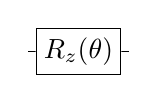
\begin{tikzpicture}
            \begin{yquant}
                qubit {} q[1];
                box {\(R_z(\theta)\)} q[0];
            \end{yquant}
        \end{tikzpicture}
        \fi} \\[1em]
        Faasinihe & \(P(\lambda)\) & \(
        \begin{pmatrix}
            1 & 0 \\
            0 & e^{i\lambda} \\
        \end{pmatrix}
        \) & \lower6pt\hbox{
        \ifdefined\yquanton
        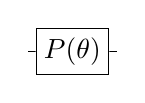
\begin{tikzpicture}
            \begin{yquant}
                qubit {} q[1];
                box {\(P(\theta)\)} q[0];
            \end{yquant}
        \end{tikzpicture}
        \fi} \\[1em]
        Juhitud eitus & \(\CNOT\) & \(
        \begin{pmatrix}
            1 & 0 & 0 & 0 \\
            0 & 0 & 0 & 1 \\
            0 & 0 & 1 & 0 \\
            0 & 1 & 0 & 0 \\
        \end{pmatrix}
        \) & \lower6pt\hbox{
        \ifdefined\yquanton
        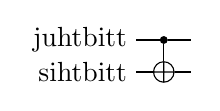
\begin{tikzpicture}
            \begin{yquant}
                qubit {juhtbitt} ctrl;
                qubit {sihtbitt} trgt;
                cnot trgt | ctrl;
            \end{yquant}
        \end{tikzpicture}
        \fi} \\
        Pauli \(X\) & \(X\) & \(
        \begin{pmatrix}
            0 & 1 \\
            1 & 0 \\
        \end{pmatrix}
        \) & \lower6pt\hbox{
        \ifdefined\yquanton
        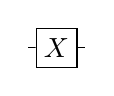
\begin{tikzpicture}
            \begin{yquant}
                qubit {} q[1];
                box {\(X\)} q[0];
            \end{yquant}
        \end{tikzpicture}
        \fi} \\[1em]
        Pauli \(Y\) & \(Y\) & \(
        \begin{pmatrix}
            0 & -i \\
            i & 0 \\
        \end{pmatrix}
        \) & \lower6pt\hbox{
        \ifdefined\yquanton
        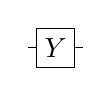
\begin{tikzpicture}
            \begin{yquant}
                qubit {} q[1];
                box {\(Y\)} q[0];
            \end{yquant}
        \end{tikzpicture}
        \fi} \\[1em]
        Pauli \(Z\) & \(Z\) & \(
        \begin{pmatrix}
            1 & 0 \\
            9 & -1 \\
        \end{pmatrix}
        \) & \lower6pt\hbox{
        \ifdefined\yquanton
        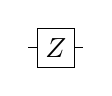
\begin{tikzpicture}
            \begin{yquant}
                qubit {} q[1];
                box {\(Z\)} q[0];
            \end{yquant}
        \end{tikzpicture}
        \fi} \\[1em]
        Hadamardi operaator & \(H\) & \(
        \frac{1}{\sqrt{2}} \begin{pmatrix}
            1 & 1 \\
            1 & -1 \\
        \end{pmatrix}
        \) & \lower6pt\hbox{
        \ifdefined\yquanton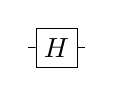
\begin{tikzpicture}
            \begin{yquant}
                qubit {} q[1];
                box {\(H\)} q[0];
            \end{yquant}
        \end{tikzpicture}
        \fi} \\[1em]
        Faasioperaator & \(S\) & \(
        \begin{pmatrix}
            1 & 0 \\
            0 & i \\
        \end{pmatrix}
        \) & \lower6pt\hbox{
        \ifdefined\yquanton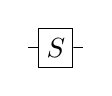
\begin{tikzpicture}
            \begin{yquant}
                qubit {} q[1];
                box {\(S\)} q[0];
            \end{yquant}
        \end{tikzpicture}
        \fi} \\[1em]
        Pöördfaasioperaator & \(S^{\dagger}\) & \(
        \begin{pmatrix}
            1 & 0 \\
            0 & -i \\
        \end{pmatrix}
        \) & \lower6pt\hbox{
        \ifdefined\yquanton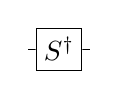
\begin{tikzpicture}
            \begin{yquant}
                qubit {} q[1];
                box {\(S^{\dagger}\)} q[0];
            \end{yquant}
        \end{tikzpicture}
        \fi} \\[1em]
        Bittide vahetus & \(\SWAP\) & \(
        \begin{pmatrix}
            1 & 0 & 0 & 0 \\
            0 & 0 & 1 & 0 \\
            0 & 1 & 0 & 0 \\
            0 & 0 & 0 & 1 \\
        \end{pmatrix}
        \) & \lower6pt\hbox{
        \ifdefined\yquanton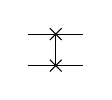
\begin{tikzpicture}
            \begin{yquant}
                qubit {} q[2];
                swap (q[0, 1]);
            \end{yquant}
        \end{tikzpicture}
        \fi} \\
        \midrule
        Mõõtmine & --- & --- & \lower6pt\hbox{
        \ifdefined\yquanton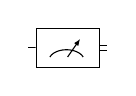
\begin{tikzpicture}
            \begin{yquant}
                qubit {} q[1];
                measure q[0];
            \end{yquant}
        \end{tikzpicture}
        \fi} \\
        \bottomrule
    \end{tabular}
    \caption{Töös kasutatud operaatorid, nende tähistused, definitsioonid ja tähitused ahelas~\cite{nielsen+chuang, kaye+laflamme+mosca}}
    \label{tab:gates}
\end{table}

Võimalike kvantväravaid on lõpmatu arv, kuid on riistvaras vaja realiseerida vaid mõned väravad, mis moodustavad univeraalse komplekti.
Kõik teised väravad saab esitada univeraalse komplekti kaudu~\cite{mcardle+etal, nielsen+chuang, kaye+laflamme+mosca}.

Univeraalseid komplekte on lõpmata palju.
Komplektis peab alati olema põimiv värav.
Tihti võetakse põimivaks väravaks juhitud eitus ja kõik algoritmid esitatakse juhitud eituse kaudu, nagu ka siin töös~\cite{mcardle+etal, nielsen+chuang, kaye+laflamme+mosca}.

Juhitud väravad on sellised, mis rakenduvad sihtbitile vaid sel määral, mil
määral juhtbitt on olekus \(\ket1\), juhtibitti muutmata. Näiteks
\begin{align}
    \CNOT \paren{\alpha \ket{0} \otimes \ket{1} + \beta \ket{1} \otimes \ket{1}}
    = \alpha \ket{0} \otimes \ket{1} + \beta \ket{1} \otimes \ket{0} \rlap{.}
\end{align}
Töös kasutatud juhitud väravaid pole enamasti tabelis~\ref{tab:gates} eraldi toodud.

Mõõtmine pole unitaarne operatsioon ja sellega ei seostu väravat. Siiski
tähistatakse ahelates seda väravatega sarnaselt. Tabelis~\ref{tab:gates} on
tähistus toodud. Definitsiooni pole toodud.

Kvantäravate järjestuse ja bittidele rakendamise korra määrab kvantahel.
Joonis~\ref{fig:circuits} on näide ahelast. Igat üksikut biti või registrit
tervikuna tähistab horisontaalne traat. Traadist vasakul on sisend- ja paramal
väljundolekud, kui need on olulised. Operaatorid on kastid. Operaator rakendub
igale bitile, mille traat kasti läbib. Katsutid (punktiga lõppevad vertikaalsed
jooned) ühendavad operaatoreid juhtbitide või juhtregistritega, kui neid on.

\begin{figure}
    \centering
    \ifdefined\yquanton
    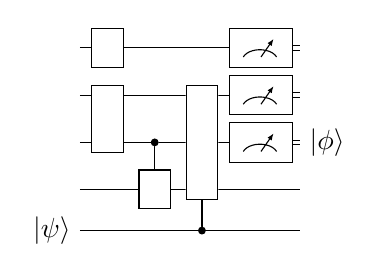
\begin{tikzpicture}
        \begin{yquant}
            qubit {} q[4];
            qubit {\(\ket{\psi}\)} q[+1];
            box {} q[0];
            box {} (q[1, 2]);
            box {} q[3] | q[2];
            box {} (q[1, 2, 3]) | q[4];
            measure q[0, 1, 2];
            output {\(\ket{\phi}\)} q[2];
        \end{yquant}
    \end{tikzpicture}
    \fi
    \caption{Kvantahela näide}
    \label{fig:circuits}
\end{figure}

Pikemalt tutvutavad ahelamudelit \cite{nielsen+chuang} ja
\cite{kaye+laflamme+mosca}. Samas \cite{cao+etal} ja \cite{mcardle+etal} on
põgusamad tutvustused, kuid suunatud just kvantsimulatsioonile.

Selles töös on keskne faasi hindamise algoritm, mis on klassikalisest analoogist efektiivsem.
Kokkuhoiu teevad võimalikuks kaks kvantarvutuse olulist võtet: kvantparallelism ja põimituse kasutamine.

Kvantparallelism põhineb operaatorite lineaaruselt, mis tähendab, et korraga on võimalik arvutada operaatori mõju mitmel juhul:
\begin{align}
    U \paren{\alpha\ket{0} + \beta\ket{1}}
    = \alpha U \ket{0} + \beta U \ket{1} \rlap{.}
\end{align}
Tõsi, tulemuste välja lugemiseks tuleb kvantarvuti programmi käitada mitu korda~\cite{mcardle+etal}.

Põimituse kasulikust lühidalt kokku võtta ei saa: see on igas algoritmis isemoodi.

Kvantparallelismi ja põimitust ei õnnestu klassikaliselt efektiivselt simuleerida.
Sestap on neid ülesande efektiivsemaks lahendamiseks võimalik ära kasutada vaid kvantarvuteid.

\textbf{Üle kontrollida:} Põimituse klassikaline simuleerimine on näide tugevalt korreleeritud probleemist.
Et ka mitmed kvantkeemia ja -füüsika probleemid on tugevalt korreleeritud, siis arvatakse, et nende lahendamiseks sobivad just kvantarvutid~\cite{cao+etal}.

\section{Faasi hindamise algoritm}\label{sec:pea}

Selles alapeatükis keskendume faasi hindamise algoritmile.

Jaotises~\ref{sec:qft} käsitleme faasi hindamise algoritmi ühte põhilist osa: kvantarvutusliku Fourier' teisendust.

Jaotises~\ref{sec:unit} esitame faasi hindamise algoritmi enese, keskendudes selle peamisele kasutusjuhule, milleks on unitaarse operaatori omaväärutste leidmine.

Jaotises~\ref{sec:hermit} näitame, kuidas faasi hindamise algoritmi õnnestub kasutada ka hermiitiliste operaatorite omaväärtuste leidmiseks.
Viimane rakendus pakub meile huvi, sest hamiltoniaan on hermiitiline operaator.

\(\subsection{Kvantarvutuslik Fourier' teisendus ja pöördteisendus}\label{sec:qft}

Kvantarvutusliku Fourier' teisenduse algoritm ja pöördteisenduse algoritm on faasi hindamise algoritmi tähtsad osad.
Vaatame nende tööpõhimõtet.

Kvantarvtusliku Fourier' teisenduse definitsioon on
\begin{align}\label{f:qftdef}
    \QFT\colon
    \ket{j} \mapsto \frac{1}{\sqrt{2^n}} \sum_{k=0}^{2^n-1} e^{2\pi ijk/2^n} \ket{k} \rlap{,}
\end{align}
kus \(\ket{j}\) ja \(\ket{k}\) \(n\)-kvantbitised
baasivektorid. Et tegemist on lineaarse operatsiooniga, siis piisab käsitleda selle mõju baasivektoritele~\cite{nielsen+chuang, kaye+laflamme+mosca}.

\begin{figure}
    \centering
    \ifdefined\yquanton
    \begin{tikzpicture}[scale=0.8]
        \begin{yquant}
            qubit {\(\ket{j_1}\)} q[1];
            qubit {\(\ket{j_2}\)} q[+1];
            qubit {\(\vdots\)} q[+1]; discard q[2];
            qubit {\(\ket{j_{n-1}}\)} q[+1];
            qubit {\(\ket{j_n}\)} q[+1];
            h q[0];
            box {\(P(2\pi/2^2)\)} q[0] | q[1];
            text {\(\ \ldots\ \)} q[0, 1, 3, 4];
            h q[1];
            text {\(\ \ldots\ \)} q[0, 1, 3, 4];
            box {\(P(2\pi/2^{n-2})\)} q[1] | q[3];
            box {\(P(2\pi/2^{n-1})\)} q[1] | q[4];
            text {\(\ \ldots\ \)} q[0, 1, 3, 4];
            h q[3];
            box {\(P(2\pi/2^2\)} q[3] | q[4];
            h q[4];
            swap (q[0, 4]);
            swap (q[1, 3]);
            output {\(\frac{\ket0+e^{2\pi0.j_n}\ket1}{\sqrt{2}}\)} q[0];
            output {\(\frac{\ket0+e^{2\pi0.j_{n-1}j_n}\ket1}{\sqrt{2}}\)} q[1];
            output {\(\vdots\)} q[2];
            output {\(\frac{\ket0+e^{2\pi0.j_2\cdots j_n}\ket1}{\sqrt{2}}\)} q[3];
            output {\(\frac{\ket0+e^{2\pi0.j_1\cdots j_n}\ket1}{\sqrt{2}}\)} q[4];
        \end{yquant}
    \end{tikzpicture}
    \fi
    \caption{Kujutatud on kvantarvutusliku Fourier' teisenduse ahel~\cite{nielsen+chuang, kaye+laflamme+mosca}.}
    \label{fig:qft}
\end{figure}

Näitame, et kvantarvutusliku Fourier' teisenduse realiseerib ahel joonisel~\ref{fig:qft}.

Edasipidi asutame tähistust, kus
\begin{multline}
    j_1j_2\cdots j_n.j_{n+1}j_{n+2}\cdots j_m \\
    = j_1 2^{n-1} j_2 2^{n-2} + \cdots + j_n 2^0 + j_{n+1} 2^{-1} j_{n+2} 2^{-2} + \cdots j_m 2^{-m} \rlap{,}
    \qquad j_i \in \{0, 1\} \rlap{.}
\end{multline}
Selles ja järgmises jaotises on kõik komaga arvud kahendmurrud (mitte kümnendmurrud).

On vaja teada, et Hadamardi operaatori mõju baasvektoritele on
\begin{align}
    H\ket{0} = \frac{\ket{0} + \ket{1}}{\sqrt{2}}
\end{align}
ja
\begin{align}
    H\ket{1} = \frac{\ket{0} - \ket{1}}{\sqrt{2}} \rlap{.}
\end{align}
Viimased kaks tingimust saab kokku võtta üheks
\begin{align}
    H\ket{j_i} = \frac{\ket{0} + e^{2\pi i0.j_i}\ket{1}}{\sqrt{2}}\rlap{.}
\end{align}

Samuti on vaja teada, et parameetriga faasioperaatori mõju baasivektoritele on
\begin{align}
    P(\lambda)\ket{0} = \ket{0}
\end{align}
ja
\begin{align}
    P(\lambda)\ket{1} = e^{i\lambda}\ket{0} .
\end{align}
Viimasest kahest tingimusest järeldub kasulik omadus
\begin{align}\label{f:phase}
    P(2\pi i0.0j_2) = \frac{\ket{0} + e^{2\pi i 0.j_1} \ket{1}}{\sqrt{2}}
    = \frac{\ket{0}+e^{2\pi i0.j_1j_2}\ket{1}}{\sqrt{2}} .
\end{align}

Järgime joonise~\ref{fig:qft} ahela loogikat samm-sammult.

Algolek on
\begin{align}
    \ket{j_1} \otimes \ket{j_2} \otimes \cdots \otimes \ket{j_n} \rlap{.}
\end{align}

Kõigepealt tuleb esimesele kvantbitile mõjuda Hadamardi operaatoriga \(H\).
Pärast seda on olek
\begin{align}
    \frac{\ket{0} + e^{2\pi i0.j_1}\ket{1}}{\sqrt{2}} \otimes \ket{j_2} \otimes \cdots \otimes \ket{j_n} \rlap{.}
\end{align}

Järgmiseks tuleb mõjuda esimesele kvantbittile faasiväravaga \(P(2\pi/2^2)\) juhinduvalt teisest kvantbitist.
Kui \(j_2 = 0\), siis esimest bitti ei mõjutata, mis on sama hea, kui mõjuda operaatoriga \(P(2\pi 0.00)\).
Kui \(j_2 = 1\), siis mõjutakse operaatoriga \(P(2\pi 0.01)\).
Kokkuvõttes võib öelda, et teisele bitile mõjutakse operaatoriga \(P(2\pi 0.0j_2)\).
Tulenevalt valemist~\ref{f:phase} on pärast seda olek
\begin{align}
    \frac{\ket{0} + e^{2\pi i0.j_1j_2}\ket{1}}{\sqrt{2}} \otimes \ket{j_2} \otimes \cdots \otimes \ket{j_n} \rlap{.}
\end{align}

Edasi tuleb mõjuda esimesele kvantbitile faasiväravaga \(P(2\pi/2^3)\) juhinduvalt kolmandast kvantbitist.
Tulemuseks on
\begin{align}
    \frac{\ket{0} + e^{2\pi i0.j_1j_2j_3}\ket{1}}{\sqrt{2}} \otimes \ket{j_2} \otimes \cdots \otimes \ket{j_n} \rlap{.}
\end{align}

Sarnaselt tuleb toimida ka juhinduvalt ülejäänud kvantbititdest.
Lõpuks on tulemuseks
\begin{align}
    \frac{\ket{0} + e^{2\pi i0.j_1j_2\cdots j_n}\ket{1}}{\sqrt{2}} \otimes \ket{j_2} \otimes \cdots \otimes \ket{j_n} \rlap{.}
\end{align}

Järgmiseks, teise kvantbitiga tuleb toimida analoogselt esimesega.
Seejärel on olek
\begin{align}
    \frac{\ket{0} + e^{2\pi i0.j_1j_2\cdots j_n}\ket{1}}{\sqrt{2}}
    \otimes \frac{\ket{0} + e^{2\pi i0.j_2j_3\cdots j_n}\ket{1}}{\sqrt{2}}
    \otimes \ket{j_3} \otimes \cdots \otimes \ket{j_n} \rlap{.}
\end{align}

Kui sama skeemi järgida ülejäänud bitte jaoks, on lõpuks olek
\begin{align}
    \frac{\ket{0} + e^{2\pi i0.j_1j_2\cdots j_n}\ket{1}}{\sqrt{2}}
    \otimes \frac{\ket{0} + e^{2\pi i0.j_2j_3\cdots j_n}\ket{1}}{\sqrt{2}}
    \otimes \cdots
    \otimes \frac{\ket{0} + e^{2\pi i0.j_n}\ket{1}}{\sqrt{2}} \rlap{.}
\end{align}

Viimaks tuleb bittide järjekorda vahetada.
Tulemuseks on
\begin{align}\label{f:qftfinal}
    \frac{\ket{0} + e^{2\pi i0.j_n}\ket{1}}{\sqrt{2}}
    \otimes \frac{\ket{0} + e^{2\pi i0.j_{n-1}j_n}}{\sqrt{2}}
    \otimes \cdots
    \otimes \frac{\ket{0} + e^{2\pi i0.j_1j_2\cdots j_n}\ket{1}}{\sqrt{2}} \rlap{.}
\end{align}

Avades sulud ja koondades, saab oleku~\ref{f:qftfinal} kirja panna kujul
\begin{equation}\label{f:qftfinaltrans}
    \frac{1}{\sqrt{2^n}}\sum_{k=0}2^{n-1}e^{2\pi ijk/2^n}\ket k \rlap{,}
\end{equation}
milline peabki olema Fourier' teisenduse tulemus~\cite{nielsen+chuang, kaye+laflamme+mosca}.

Järgnevas jaotises läheb vaja ka kvantarvutusliku Fourier' pöördteisendust, mille kohaselt
\begin{align}
    \QFT^{-1}\colon
    \frac{1}{\sqrt{2^n}} \sum_{k=0}^{2^n-1} e^{2\pi ijk/2^n} \ket{k} \mapsto \ket{j} \rlap{.}
\end{align}
Pöörteisenduse ahela saamiseks tuleb teisenduse ahel pöörata: ahel tuleb koostada vastupidises järjekorras, asendades operaatorid pöördoperaatoritega~\cite{kaye+laflamme+mosca}.
Kehtivad seosed
\begin{align}
    H^{-1} &= H \rlap{,} \\
    P^{-1}(\lambda) &= P(-\lambda) \rlap{,} \\
    \SWAP^{-1} &= \SWAP \rlap{.}
\end{align}

Klassikalise Fourier' teisenduse valem on
\begin{align}\label{f:cftdef}
    y_k = \frac{1}{\sqrt{N}} \sum_{j=0}^{N-1}e^{2\pi ijk/N} x_j \rlap{.}
\end{align}
Valemite \eqref{f:qftdef} ja \ref{f:cftdef} võrdlusest selgub, et kvantarvutusliku Fourier' teisenduse käigus toimub klassikaline Fourier' teisendus, kui võtta \(N = 2^n\)~\cite{nielsen+chuang}.

Klassikaliselt on Fourier' teisendusel \(N \log{N}=n 2^n \) sammu, kvantavutuslikult vaid \(\log^2{N} = n^2\) sammu.
Pealt näha on sama ülesande lahendamine kvantarvutuslikult oluliselt efektiivsem kui klassikaliselt~\cite{nielsen+chuang}.

Paraku pole kvantarvutuslikult arvutatud klassikalise Fourier' teisenduse tulemus otseselt mõõdetav, kuivõrd see on talletatud lõppoleku amplituudidesse.
Sestap ei saa kvantarvutsliku teisendust kasutada lihtsalt klassikalise Fourier' teisenduse efektiivsema asendusena~\cite{nielsen+chuang}.

Siiski õnnestub kvantarvtusliku Fourier' teisendust kasutada teatud ülesannete klassikalisest efektiivsemaks lahendamiseks.
Antud töö jaoks on oluline, et see leiab kasutust faasi hindamise algoritmis, mida tutvustab järgmine jaotis.

\subsection{Unitaarse operaatori omaväärtuste leidmine}\label{sec:unit}

Unitaarse operaatori \(U\) jaoks kehtib omaväärtusvõrrand
\begin{align}
    U\ket{\Psi} = e^{2\pi i\phi}\ket{\Psi} \rlap{,}
    \qquad \phi \in [0,1) \rlap{,}
\end{align}
kus \(\ket{\Psi}\) on meid huvitav olek ja \(e^{2\pi i\phi}\) omaväärtus, mida kutsutakse ka faasiks.
Faasi hindamise algoritm võimaldab leida parameetri \(\phi\), millega on faas määratud.

Näitame, et ülesande lahendamiseks sobib ahel joonisel~\ref{fig:pea}.

\begin{figure}[h]
    \centering
    \ifdefined\yquanton
    \begin{tikzpicture}
        \begin{yquant}
            qubit {$\ket0$} pea[1];
            qubit {$\ket0$} pea[+1];
            qubit {$\vdots$} pea[+1]; discard pea[2];
            qubit {$\ket0$} pea[+1];
            qubit {$\ket0$} pea[+1];
            qubit {$\ket u$} state;
            box {$\mathop{\rm QFT}$} (pea[0], pea[1], pea[2], pea[3], pea[4]);
            box {$U^{2^0}$} state | pea[4];
            box {$U^{2^1}$} state | pea[3];
            text {$\ \ldots\ $} pea[0], pea[1], pea[3], pea[4], state;
            box {$U^{2^{n-2}}$} state | pea[1];
            box {$U^{2^{n-1}}$} state | pea[0];
            box {$\mathop{\rm QFT}\nolimits^{-1}$} (pea[0], pea[1], pea[2], pea[3], pea[4]);
            measure pea[0], pea[1], pea[3], pea[4];
            output {$\phi_1$} pea[0];
            output {$\phi_2$} pea[1];
            output {$\vdots$} pea[2];
            output {$\phi_{n-1}$} pea[3];
            output {$\phi_n$} pea[4];
            output {$\ket u$} state;
        \end{yquant}
    \end{tikzpicture}
    \fi
    \caption{Kvantahel \(U\) faasi hindamiseks \cite{nielsen+chuang, kaye+laflamme+mosca}}
    \label{fig:pea}
\end{figure}

Joonise~\ref{fig:pea} ahelas on kaks kvantregistrit.
Tööregistrit kujutavad ülemised \(n\) traati.
Kõige alumine traat on olekuregister.%
\footnote{Kuigi olekuregistrit on kujutatud vaid ühe traadiga, võib selles olla kuitahas palju kvantbitte.}

Järgime joonise~\ref{fig:pea} ahela loogikat samm-sammult.

Joonisel~\ref{fig:pea} on eeldatud, et olekuregister on juba \(U\) omaolekus
\(\ket{u}\), praktikas tuleb see olek kuidagi ette valmistada.

Esimese sisulise sammuna tuleb faasi hindamise registrile mõjuda kvantarvutusliku Fourier' teisenduse väravaga.
Selle värava realiseerib eelmises jaotises esitatud ahel.
Kui faasi hindamise registri kvantbitid olid enne kvantarvutusliku Fourier' teisenduse värava rakendamise järel on tulemuseks olek
\begin{align}\label{f:peainit}
    \underbrace{\frac{\ket{0}+\ket{1}}{\sqrt{2}}
    \otimes \cdots
    \otimes \frac{\ket{0}+\ket{1}}{\sqrt{2}}}_n
    \otimes \ket{u} \rlap{.}
\end{align}

Järgmisena tuleb olekuregistile mõjuda operaatoriga \(U^{2^0}\) juhinduvalt faasi hindasmie registri viimasest bitist.
Selle tulemuseks on olek
\begin{align}\label{f:peau0}
    \underbrace{\frac{\ket{0}+\ket{1}}{\sqrt{2}}
    \otimes \cdots
    \otimes \frac{\ket{0}+\ket{1}}{\sqrt{2}}}_{n - 1}
    \otimes \frac{\ket{0}+e^{2\pi i2^0\phi}\ket{1}}{\sqrt{2}}
    \otimes \ket{u} \rlap{.}
\end{align}

Veendume selles võttes \(\ket{u} = \alpha\ket{0} + \beta\ket{1}\).
Siis oleku~\ref{f:peainit} saab kirja panna kujul
\begin{multline}
    \underbrace{\frac{\ket{0}+\ket{1}}{\sqrt{2}}
    \otimes \cdots
    \otimes \frac{\ket{0}+\ket{1}}{\sqrt{2}}}_n
    \otimes \paren{\alpha \ket{0} + \beta \ket{1}} \\
    = \underbrace{\frac{\ket{0}+\ket{1}}{\sqrt{2}}
    \otimes \cdots
    \otimes \frac{\ket{0}+\ket{1}}{\sqrt{2}}}_{n - 1}
    \otimes \frac{1}{\sqrt{2}} \paren{
        \alpha \ket{00} + \alpha \ket{10}
        + \beta \ket{01} + \beta \ket{11}
    } \rlap{.}
\end{multline}
Uus olek on
\begin{multline}
    \underbrace{\frac{\ket{0}+\ket{1}}{\sqrt{2}}
    \otimes \cdots
    \otimes \frac{\ket{0}+\ket{1}}{\sqrt{2}}}_{n - 1}
    \otimes \frac{1}{\sqrt{2}} \paren{
        \alpha \ket{00} + \alpha U^{2^0} \ket{10}
        + \beta \ket{01} + \beta U^{2^0} \ket{11}
    } \\
    = \underbrace{\frac{\ket{0}+\ket{1}}{\sqrt{2}}
    \otimes \cdots
    \otimes \frac{\ket{0}+\ket{1}}{\sqrt{2}}}_{n - 1}
    \otimes \frac{1}{\sqrt{2}} \paren{
        \alpha \ket{00} + \alpha e^{2\pi i2^0\phi} \ket{10}
        + \beta \ket{01} + \beta e^{2\pi i2^0\phi} \ket{11}
    } \\
    = \underbrace{\frac{\ket{0}+\ket{1}}{\sqrt{2}}
    \otimes \cdots
    \otimes \frac{\ket{0}+\ket{1}}{\sqrt{2}}}_{n - 1}
    \otimes \frac{\ket{0} + e^{2\pi i\phi 2^0} \ket{1}}{\sqrt{2}}
    \otimes \paren{\alpha \ket{0} + \beta \ket{1}} \rlap{,}
\end{multline}
mis ongi olek~\ref{f:peau0}.

Edasi tuleb olekuregistrile mõjuda operaatoriga \(U^{2^1}\) juhinduvalt faasi hindamise registri eelviimasest bitist.
Peale seda on olek
\begin{align}
    \underbrace{\frac{\ket{0} + \ket{1}}{\sqrt{2}}
    \otimes \cdots
    \otimes \frac{\ket{0} + \ket{1}}{\sqrt{2}}
    }_{n-2}
    \otimes \frac{\ket{0} + e^{2\pi i2^1\phi} \ket{1}}{\sqrt{2}}
    \otimes \frac{\ket{0} + e^{2\pi i2^0\phi} \ket{1}}{\sqrt{2}}
    \otimes \ket{u} \rlap{.}
\end{align}

Sama skeemi järgi tuleb jätkata.
Lõpuks on tulemuseks
\begin{align}\label{f:peauend}
    \frac{\ket{0}+ e^{2\pi i2^{n-1}\phi}}{\sqrt{2}}
    \otimes \frac{\ket{0}+ e^{2\pi i2^{n-2}\phi}}{\sqrt{2}}
    \otimes\cdots
    \otimes \frac{\ket{0}+ e^{2\pi i2^0\phi}}{\sqrt{2}}
    \otimes\ket{u}
\end{align}

Kui tähistada \(\phi=0.\phi_1\phi_2\cdots\phi_n\), siis võtab olek~\ref{f:peauend} kuju
\begin{align}
    \frac{\ket{0}+ e^{2\pi i0.\phi_n}\ket{1}}{\sqrt{2}}
    \otimes \frac{\ket{0}+ e^{2\pi i0.\phi_{n-1}\phi_n}\ket{1}}{\sqrt{2}}
    \otimes\cdots
    \otimes \frac{\ket{0}+ e^{2\pi i0.\phi_1\phi_2\cdots\phi_n}\ket{1}}{\sqrt{2}}
    \otimes\ket{u} \rlap{,}
\end{align}
sest
\begin{align}
    e^{2\pi i2^m\phi}
    = e^{2\pi i2^m 0.\phi_1\phi_2\cdots\phi_n}
    = e^{2\pi i0.\phi_m\phi_{m+1}\cdots\phi_n} \rlap{,}
\end{align}
globaalse faasi täpsusega.

Lõpuks tuleb faasi hindamise registrile mõjuda kvantarvutusliku Fourier' pöördteisendse väravaga.
Valemite \ref{f:qftdef}, \ref{f:qftfinal} ja \ref{f:qftfinaltrans} põhjal on tulemuseks
\begin{align}\label{f:peafinal}
    \ket{\phi_1} \otimes \ket{\phi_2} \otimes \cdots \otimes \ket{\phi_n} \otimes \ket{u} \rlap{.}
\end{align}

Kui süsteem on olekus~\ref{f:peafinal}, siis faasi hindamise registri mõõtmise tulemuseks klassikaliste bittide jada
\begin{align}
    \phi_1, \phi_2, \cdots, \phi_n \rlap{,}
\end{align}
millega on \(\phi = 0.\phi_1\phi_2 \cdots \phi_n\) määratud.

Äsja arutlesime eeldusel, et faasi hindamise registris on sama palju bitte \(n\), kui on vaja \(\phi = 0.\phi_1\phi_2 \cdots \phi_m\) esitamiseks kahendsüsteemis \(m = n\).
Praktilisel kaalutlustel ei pruugi see nii olla: \(m\) väärtus ei ole ette teada, faasi hindamiseks on kasutada piiratud arv bitte \(n < m\).

Kui \(n > m\), jääb eelnenud arutelu kehtima, ainult et \(\phi_{m+1}, \phi_{m+2}, \phi_n = 0\).

Saab näidata, et juhul, kui \(n < m\), on suurima mõõtmistõenõosusega tulemuseks \(\phi\) hinnang \(n\)-bitise täpsusega~\cite{kaye+laflamme+mosca}.
Suurima tõenõosusega kehtib
\begin{equation}
    0.\phi_1\phi_2\cdots\phi_n \in [\phi - 2^{-n-1}, \phi + 2^{n+1}] \rlap{.}
\end{equation}
Seega antud skeemi saab kasutada ka juhul, kui \(m\) pole ette teada või \(n\) on piiratud.
Mõõtmis\-tulemuste seast tuleb valida kõige tõenõolisem tulemus.

Faasi hindamise algoritm on osa Shori algoritmist algarvuliste tegurite leidmiseks, mis on oluline, sest Shori algoritmi keerukus on kõigest polünoomne, võrreldes sama eesmärgi jaoks parima klassikalise algoritmiga, mille keerukus on eksponentsiaalne~\cite{cao+etal, kaye+laflamme+mosca}.
Järeldus on, et faasi hindamise algoritm võimalab mõnesid ülesandeid klassikalisest efektiivsemalt lahendada.

Antud töös kasutme faasi hindamise algoritmi hamiltoniaani omaväärtuste leidmiseks, mis on elektronstruktuuri ülesande lahendamise kulukas.
Järgmises jaotises käistleme seda ülesanne üldise juhul: hermiitilise operaatori omaväärtuste leidmist.


\section{Hamiltoniaani simuleerimine}

Nägime, et faasi hindamise algoritmi rakendamiseks tuleb koostada Focki ruumi hamiltoniaani põhjal kvantbittide ruumi ajalise arengu operaator.
Asumegi seda tegema.

\subsection{Jordan-Wigneri teisendus}\label{sec:jw}

Antud töös kasutame Focki ruumi ülesande kvantbittide ruumi kujatamiseks Jordan-Wigneri teisendust.

Selle põhimõtte on järgmine.

Seos täitearvude esituses lainefunktsiooni ja sellele vastava kvantregisrti oleku vahel on lihtsaim võimalik: täitmata orbitaalile vastab kvantbitt olekus \(\ket{0}\) ja täidetud orbitaalile kvantbitt olekus \(\ket{1}\)~\cite{mcardle+etal}.

Tuleb arvestada, et elektronid molekulaarses süsteemis on eristamatud, kuid kvantbitid kvantregistris on eristatavad~\cite{mcardle+etal}.
Seda tehakse järgmiselt.

Hamiltoniaani kodeerimiseks seostatakse Focki ruumi tekke- ja kaoperaatorid \(\cparen{a_i, a_i^\dagger}\) kvantbittide ruumi Pauli operaatoritega \(\cparen{I, X, Y, Z}\) sedasi, et
\begin{align}
    a_j &\mapsto I^{\otimes j-1} \otimes \frac{X+iY}{2} \otimes Z^{N-j-1} \rlap{,} \\
    a_j^\dagger &\mapsto I^{\otimes j-1} \otimes \frac{X-iY}{2} \otimes Z^{N-j-1} \rlap{,}
\end{align}
misjuhul vasakul olevate operaatorite vahel kehtivad needsamad kommutatsioonireeglid, mis paremal olevate vasakul olevate vahel, vt valem~\eqref{eq:comrules}~\cite{mcardle+etal}.

Oluline on, et sellisel teisendusel on hamiltoniaani omaväärtused invariantsed.
Sestap taandubki molekulaarsete energiate leidmise ülesanne hamiltoniaani omaväärtuste leidmisele.

Jordan-Wigneri teisendus tulemusel on hamiltoniaan kujul
\begin{align}\label{eq:paulisum}
    H = \sum_i c_i h_i \rlap{,}
\end{align}
kus \(c_i\) on reaalsed konstandid ja \(h_i\) on Pauli sõned~\cite{whitfield+etal}.

Pauli sõnede all mõistame Pauli operaatorite tensorkorrutisi.

Edaspidi tähistame Pauli sõnesesid lühidalt
\begin{equation} h_i=P_{j_1}P_{j_2}\cdots P_{j_k} \rlap{,}\end{equation}
kus \(j_1\), \(j_2\), $\ldots$, \(j_k\) tähistavad kvantbitte, millele \(P_{j_1}\), \(P_{j_2}\), \(\ldots\), \(P_{j_k}\in\{X,Y,Z\}\) mõjuvad.
Näiteks \(X_1Y_2Z_4=X\otimes Y\otimes I\otimes Z.\)
(Selles tähistuses peab Pauli sõne dimensioon olema selge kontekstist, sest viimase Pauli \(X\), \(Y\) või \(Z\) operaatori järel võib olla kuitahes palju ühikmaatrikseid.)

\subsection{Trotteriseerimine ja treppalgoritm}\label{sec:qcirc}

Faasi hindamise algoritmi rakendamiseks on vaja hamiltoniaani põhjal konstrueerida ajalise arengu operaator.
Arvetades valemit~\eqref{eq:paulisum} on see
\begin{align}
    U = e^{-iHt} = e^{-it\sum_i h_i} \rlap{.}
\end{align}

Kui operaatorid \(h_i\) on kommuteeruvad, siis kehtib
\begin{align}
    e^{-it\sum_i h_i} = \prod_i e^{-i h_i t} \rlap{.}
\end{align}

Üldisemat tingimust
\begin{align}
    e^{-it\sum_i h_i}
    = \lim_{\Delta t \rightarrow 0} \paren{\prod_i e^{-i h_i \Delta t}}^{t / \Delta t} \rlap{,}
\end{align}
mis kehtib ka mittekommuteeruvate operaatorite \(h_i\) jaoks, nimetatakse Trotteri valemiks~\cite{whitfield+etal}.

Trotteriseerimiseks nimetatakas lähendust
\begin{align}\label{eq:trot}
    e^{-it\sum_i h_i}
    \approx \paren{\prod_i e^{-i h_i \Delta (t / n)}}^n \rlap{,}
\end{align}
kus \(n\) on piisavalt suur toretterisammude arv~\cite{whitfield+etal, nielsen+chuang}.

Et operaatorite korrutamine tähendab väravate järjesikku rakendamist ja täisarvuga astendamine taandub korrutamisele, on operaatori \(e^{-i t \sum_i h_i}\) realiseerimiseks kvantahelane vaja realiseerida üksikud liikmed \(e^{-i h_i a}\), kus \(a = t /n \rightarrow 0\).

Seda võimaldab nn treppalgoritm~\cite{mansky+etal}.
Vaatame selle põhimõtet.

Lihtsaim juht on
\begin{equation}\label{eq:onlyz}
  h_i = Z_{j_1}Z_{j_2}\cdots Z_{j_n} \rlap{.}
\end{equation}
Operaator \(e^{-i h_i a}\) realiseerib siis kvantahel joonisel~\ref{f:expz}.

\begin{figure}[h]
  \centering
  \ifdefined\yquanton
  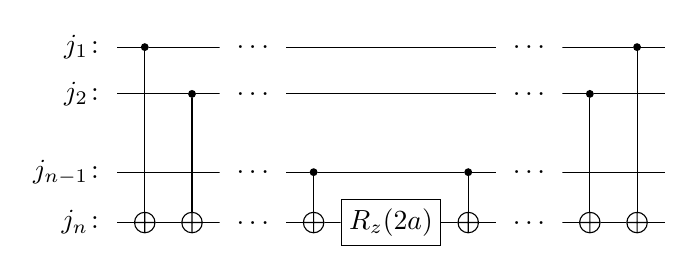
\begin{tikzpicture}
    \begin{yquant}
      qubit {$j_1\colon$} q[1];
      qubit {$j_2\colon$} q[+1];
      qubit {} q[+1]; discard q[2];
      qubit {$j_{n-1}\colon$} q[+1];
      qubit {$j_n\colon$} q[+1];
      cnot q[4] | q[0];
      cnot q[4] | q[1];
      text {$\ \ldots\ $} q[0,1,3,4];
      cnot q[4] | q[3];
      box {$R_z(2a)$} q[4];
      cnot q[4] | q[3];
      text {$\ \ldots\ $} q[0,1,3,4];
      cnot q[4] | q[1];
      cnot q[4] | q[0];
    \end{yquant}
  \end{tikzpicture}
  \fi
  \caption{Operaatori \(e^{-iZ_{j_1}Z_{j_2}\cdots Z_{j_n}a}\) realiseerimine kvantahelana~\cite{mansky+etal, nielsen+chuang}. Bitte, mis \(j_1\), \(j_2\), \(\cdots\), \(j_n\) hulgas ei esine, pole näidatud}
  \label{f:expz}
\end{figure}

Teisisõnu, bitile \(j_n\) tuleb järjest rakenda bittide \(j_1\), \(j_2\), \(\cdots\), \(j_{n-1}\) juhitud eitust.
Siis tuleb bitti \(j_n\) pöörata z-telje sihis nurga \(2a\) võrra.
Viimaks tuleb bitile \(j_n\) järjest rakendada bittide \(j_{n-1}\), \(j_{n-2}\), \(\cdots\), \(j_1\) juhitud eitusi.
Bitte, mis \(j_1\), \(j_2\), \(\cdots\), \(j_n\) hulgas ei esine, ei mõjutata~\cite{mansky+etal}.

Kesksele väravale \(R_z(2a)\) eelnev juhitud eituste osa arvutab bittide \(j_1\), \(j_2\), \(\cdots\), \(j_n\) paarsuse.
Keskne värav \(R_z(2a)\) teeb sobiva pöörde.
Järgnev juhtitud eituste osa kustutab ära nüüdseks ebavajaliku informatsiooni paarsuse kohta~\cite{nielsen+chuang}.

Üldjuhul koosneb \(h_i\) nii Pauli \(I\) ja \(Z\) kui ka \(X\) ja \(Y\) operaatoritest, kuid \(h_i\) saab alati viia kujule~\eqref{eq:onlyz} rakendades sobivaid baasiteisendusi.

Vajalikud baasiteisendused on järgmised~\cite{mansky+etal, nielsen+chuang}:
\begin{align}
    Z = HXH \rlap{,}\qquad Z = S^\dagger HYHS \rlap{.}
\end{align}

Näiteks juhul, kui
\begin{equation}
  h_i = Z_1X_2Y_3 \rlap{,}
\end{equation}
realiseerib operaatori \(e^{-i h_i t}\) ahel joonisel.

\begin{figure}[h]
  \centering
  \ifdefined\yquanton
  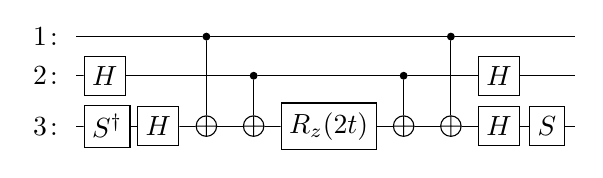
\begin{tikzpicture}
    \begin{yquant}
      qubit {$1\colon$} q[1];
      qubit {$2\colon$} q[+1];
      qubit {$3\colon$} q[+1];
      box {$H$} q[1];
      box {$S^{\dagger}$} q[2];
      box {$H$} q[2];
      cnot q[2] | q[0];
      cnot q[2] | q[1];
      box {$R_z(2t)$} q[2];
      cnot q[2] | q[1];
      cnot q[2] | q[0];
      box {$H$} q[1];
      box {$H$} q[2];
      box {$S$} q[2];
    \end{yquant}
  \end{tikzpicture}
  \fi
  \caption{\(e^{-iZ_1X_2Y_3}\) realiseerimine kvantahelana}
  \label{f:zxyex}
\end{figure}

Veel kord, operaatori \(e^{-i t \sum_i h_i}\) realiseerimiseks kvantahelana tuleb gruppide kaupa järjestiku rakendada operaatoreid \(e^{-i h_i t/n}\) realiseerivaid kvantahelaid, kus \(n\) on piisavalt suur.

Näiteks, kui
\begin{align}\label{eq:hex}
    H=\frac{1}{3}X_1Y_1+\frac{2}{3}Z_1X_2 \rlap{,}
\end{align}
ja võtta trotterisammude arvuks \(n = 2\), siis realiseerib operaatori \(e^{-i HT}\) ahel~\eqref{fig:trot}.
Lõpliku trotterisammude arvu puhul on tegemist ligikaudse hinnanguga.

\begin{figure}
    \centering
    \ifdefined\yquanton
    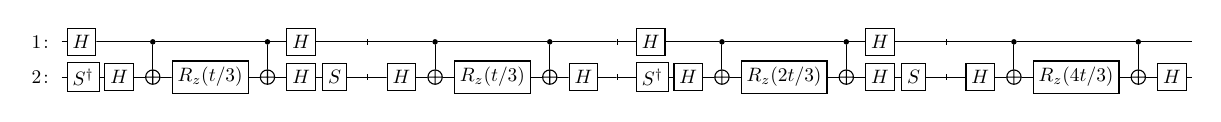
\begin{tikzpicture}[scale=0.7]
        \begin{yquant}
            qubit {$1\colon$} q[1];
            qubit {$2\colon$} q[+1];
            box {$H$} q[0];
            box {$S^\dagger$} q[1];
            box {$H$} q[1];
            cnot q[1] | q[0];
            box {$R_z(t/3)$} q[1];
            cnot q[1] | q[0];
            box {$H$} q[0];
            box {$H$} q[1];
            box {$S$} q[1];
            barrier q;
            box {$H$} q[1];
            cnot q[1] | q[0];
            box {$R_z(t/3)$} q[1];
            cnot q[1] | q[0];
            box {$H$} q[1];
            barrier q;
            box {$H$} q[0];
            box {$S^\dagger$} q[1];
            box {$H$} q[1];
            cnot q[1] | q[0];
            box {$R_z(2t/3)$} q[1];
            cnot q[1] | q[0];
            box {$H$} q[0];
            box {$H$} q[1];
            box {$S$} q[1];
            barrier q;
            box {$H$} q[1];
            cnot q[1] | q[0];
            box {$R_z(4t/3)$} q[1];
            cnot q[1] | q[0];
            box {$H$} q[1];
        \end{yquant}
    \end{tikzpicture}
    \fi
    \caption{\(e^{-i\paren{\frac{1}{3}X_1Y_1+\frac{2}{3}Z_1X_2} t} \approx \paren{e^{-i\paren{\frac{1}{3}X_1Y_1+\frac{2}{3}Z_1X_2} t/2}}^2\) realiseerimine kvantahelana-
    Joonisel on kaks operaatorite gruppi, mis vastab kahele trotterisammule.
    Igas grupis on omakorda kaks operaatorit}
    \label{fig:trotex}
\end{figure}

\subsection{Juhitud ajalise arengu operaator}

Faasihindamise jaoks on oluline, et unitaarne operaator oleks juhitud.
Juhitud unitaarse operaatori saab kui kvantahelas asendada kõik pöörded juhitud pööretega.

Nõnda toiminud, sõltub iga Pauli sõne rakendamine sellest, mis on juhtkvantbiti olek.
Kui juhtkvantbitt on olekus \(\ket0\), pööre ei rakendu.
Et paarsuse arvutamine ja selle tagasi panemine on pöördoperatsioonid, siis kokkuvõttes antud Pauli sõne eksponent justkui ei rakendu.
Kui juhtkvantvitt on olekus \(\ket1\) pööre rakendub ja rakendub ka Pauli sõne eksponent tervikuna.

Joonisel~\ref{fig:trotexctrl} on näide juhitud ajalise arengu operaatorist, kui hamiltoniaan on antud valemiga~\eqref{j:hex}.

\begin{figure}
    \centering
    \ifdefined\yquanton
    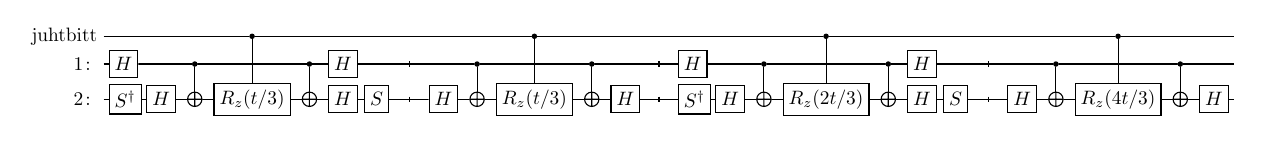
\begin{tikzpicture}[scale=0.7]
        \begin{yquant}
            qubit {juhtbitt} ctrl;
            qubit {$1\colon$} q[1];
            qubit {$2\colon$} q[+1];
            box {$H$} q[0];
            box {$S^\dagger$} q[1];
            box {$H$} q[1];
            cnot q[1] | q[0];
            box {$R_z(t/3)$} q[1] | ctrl[0];
            cnot q[1] | q[0];
            box {$H$} q[0];
            box {$H$} q[1];
            box {$S$} q[1];
            barrier q;
            box {$H$} q[1];
            cnot q[1] | q[0];
            box {$R_z(t/3)$} q[1] | ctrl[0];
            cnot q[1] | q[0];
            box {$H$} q[1];
            barrier q;
            box {$H$} q[0];
            box {$S^\dagger$} q[1] ;
            box {$H$} q[1];
            cnot q[1] | q[0];
            box {$R_z(2t/3)$} q[1] | ctrl[0];
            cnot q[1] | q[0];
            box {$H$} q[0];
            box {$H$} q[1];
            box {$S$} q[1];
            barrier q;
            box {$H$} q[1];
            cnot q[1] | q[0];
            box {$R_z(4t/3)$} q[1] | ctrl[0];
            cnot q[1] | q[0];
            box {$H$} q[1];
        \end{yquant}
    \end{tikzpicture}
    \fi
    \caption{\(e^{-i\paren{\frac{1}{3}X_1Y_1+\frac{2}{3}Z_1X_2} t} \approx \paren{e^{-i\paren{\frac{1}{3}X_1Y_1+\frac{2}{3}Z_1X_2} t/2}}^2\) realiseerimine kvantahelana-
    Joonisel on kaks operaatorite gruppi, mis vastab kahele trotterisammule.
    Igas grupis on omakorda kaks operaatorit}
    \label{fig:trotexctrl}
\end{figure}

Kui hamiltoniaanis esineb liige, mis on vaid ühikmaatriksite tensorkorrutis, tuleb seda eraldi arvestada.
Sellise liikme eksponent on globaalse faasi operaator, mille võib ajalise arengu operaatori, mis pole juhitud, juhul arvestamata jätta.
Samas juhitud globaalse faasi operaator rakendamine muudab suhtelist faasi ja seda peab arvestama.

Juhtitud globaalse faasi operaatori võib asendanda juhtkvantvitil rakendatud suhtelise faasi opetaatoriga, nagu näha joonisel~\ref{fig:globphase}, kus võrduse vasak ja parem pool on samaväärsed globaalse faasi täpsusega.

\begin{figure}[h]
    \centering
    \ifdefined\yquanton
    \begin{tikzpicture}
        \begin{yquantgroup}
            \registers{
                qubit {} q[2];
            }
            \circuit{
                box {\(GP(t)\)} q[1] | q[0];
            }
            \equals
            \circuit{
                box {\(P(-t)\)} q[0];
                barrier q[1];
            }
        \end{yquantgroup}
    \end{tikzpicture}
    \fi
    \caption{Juhitud globaalse faasi operaaotri saab asendada juhtkvantbitile rakendatud faasi operaatoriga, mille argument peab olema vastupidine~\cite{nielsen+chuang}}
    \label{fig:globphase}
\end{figure}

\chapter{Metoodika ja tulemused}\label{chap:results}

\section{Kasutatud vahendid}

Töös kasutsime programmeerimiskeelt Python.

Molekulaarsete integraalide arvutamist ja Jordan-Wigneri teisendust võimaldas teek OpenFermion~\cite{openfermion}.

Kvantahela koostamiseks ja selle klassikaliseks simuleerimiseks kasutasime teeki Qiskit~\cite{qiskit}.

Trotterisammude arvu, faasi hindamise registri suuruse ja energia piirväärtuse valikut selgitame järgmistes jaotistes.

Kasutasime keemilist baasi STO-3G.

\section{Vesiniku molekuli eneriga}

Meetodi demonsteerimiseks arvutasime vesiniku molekuli põhienergia.

Antud keemilises baasis, Jordan-Wigneri teisenduste järel, on hamiltoniaan neljakvantbitine.

Põhioleku hinnanguna kasutasime Hatree-Focki olekut
\begin{align}
    \ket{HF} = \ket{1100} \rlap{.}
\end{align}

Joonisel~\ref{fig:scan} on põhienergia sõltuvus sidemepikkusest.

Joonise~\ref{fig:scan} jaoks leitud energiad on arvutatud 10-kvantbitise täpsusega, 3 trotterisammuga.
Energia ülemiseks piiriks on võetud \(2E_h\).
Nende parameetrite valikut põhjendavad järgnevad jaotised.

\begin{figure}[h]
    \centering
    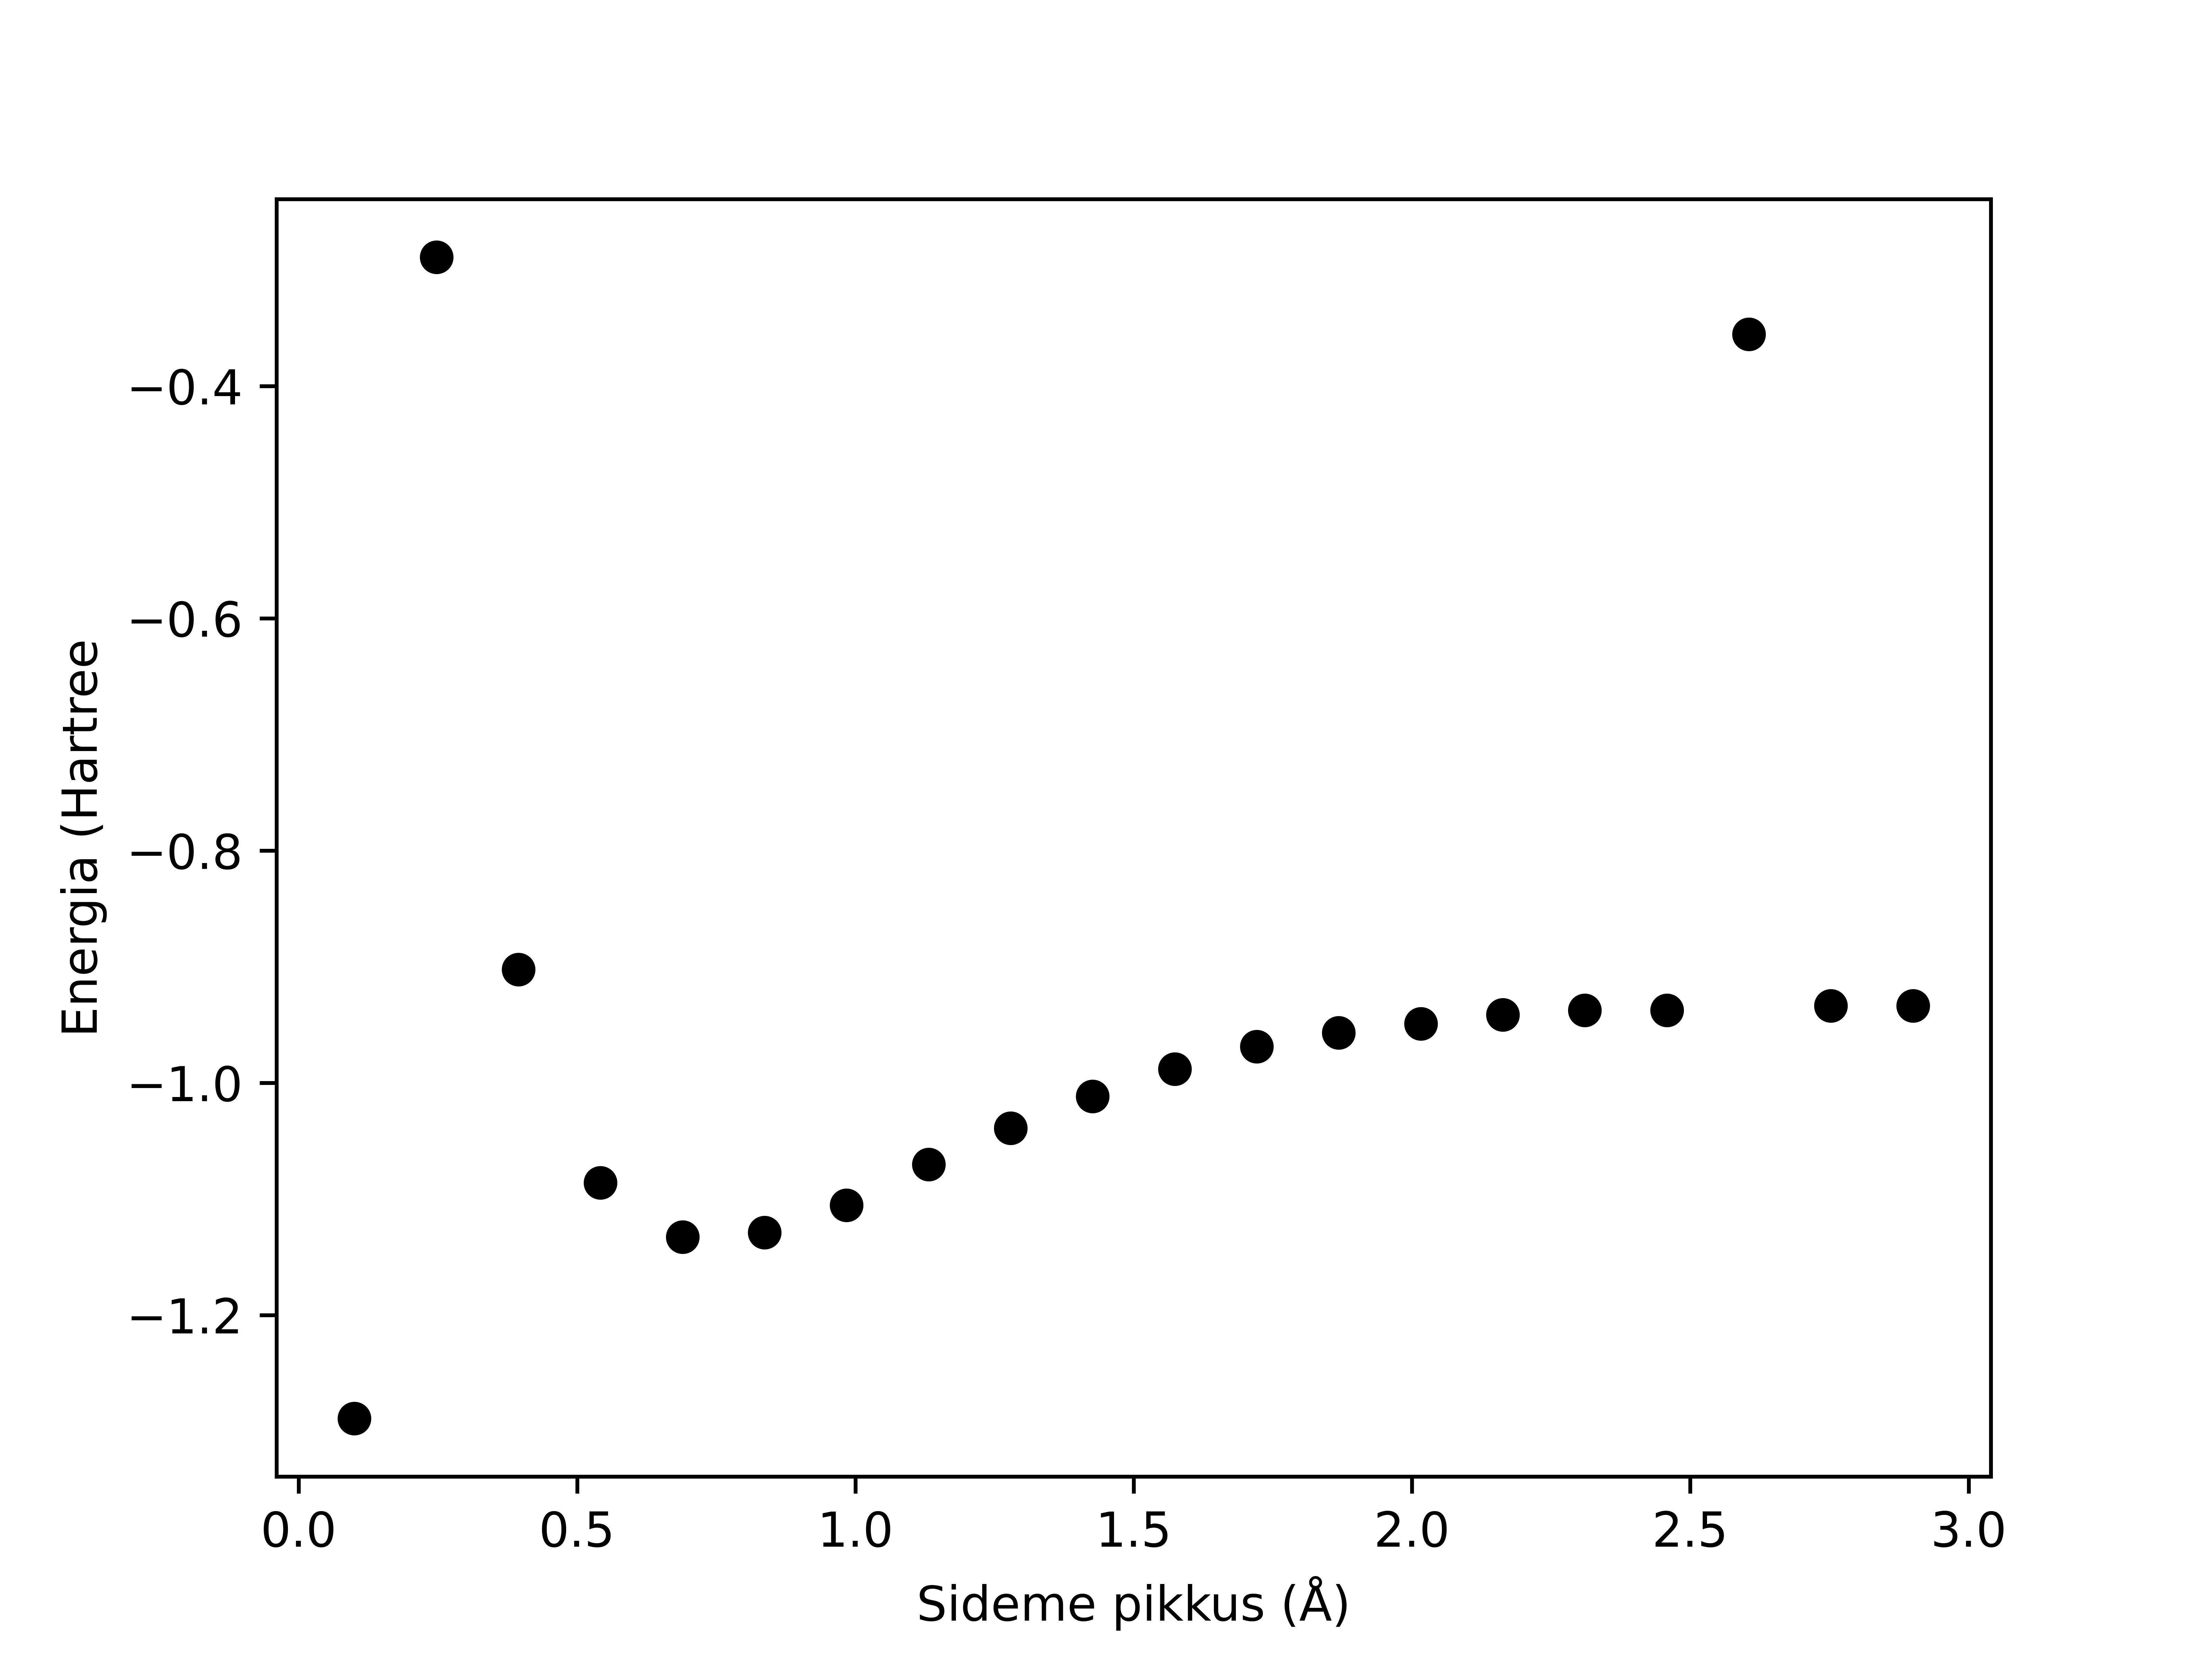
\includegraphics{scan.jpg}
    \caption{Vesiniku elektronkatte energia sõltuvus sideme pikkusest}
    \label{fig:scan}
\end{figure}

\section{Trotterisammude arv ja faasi hindamise registri suurus}

Sobivate parameetrite leidmist alustasime trotterisammude arvu määramisest.

Antud töös proovisime järjest suuremat trotterisammude arvu, kuni sammude arvu suurendamine hinnangut enam ei mõjutanud ja saavatatud oli keemiline täpsus, mis on \(0.0016E_h\).
Kvantbittide arvu piiras kvantahela käitamise aeg.

\begin{figure}[h]
    \centering
    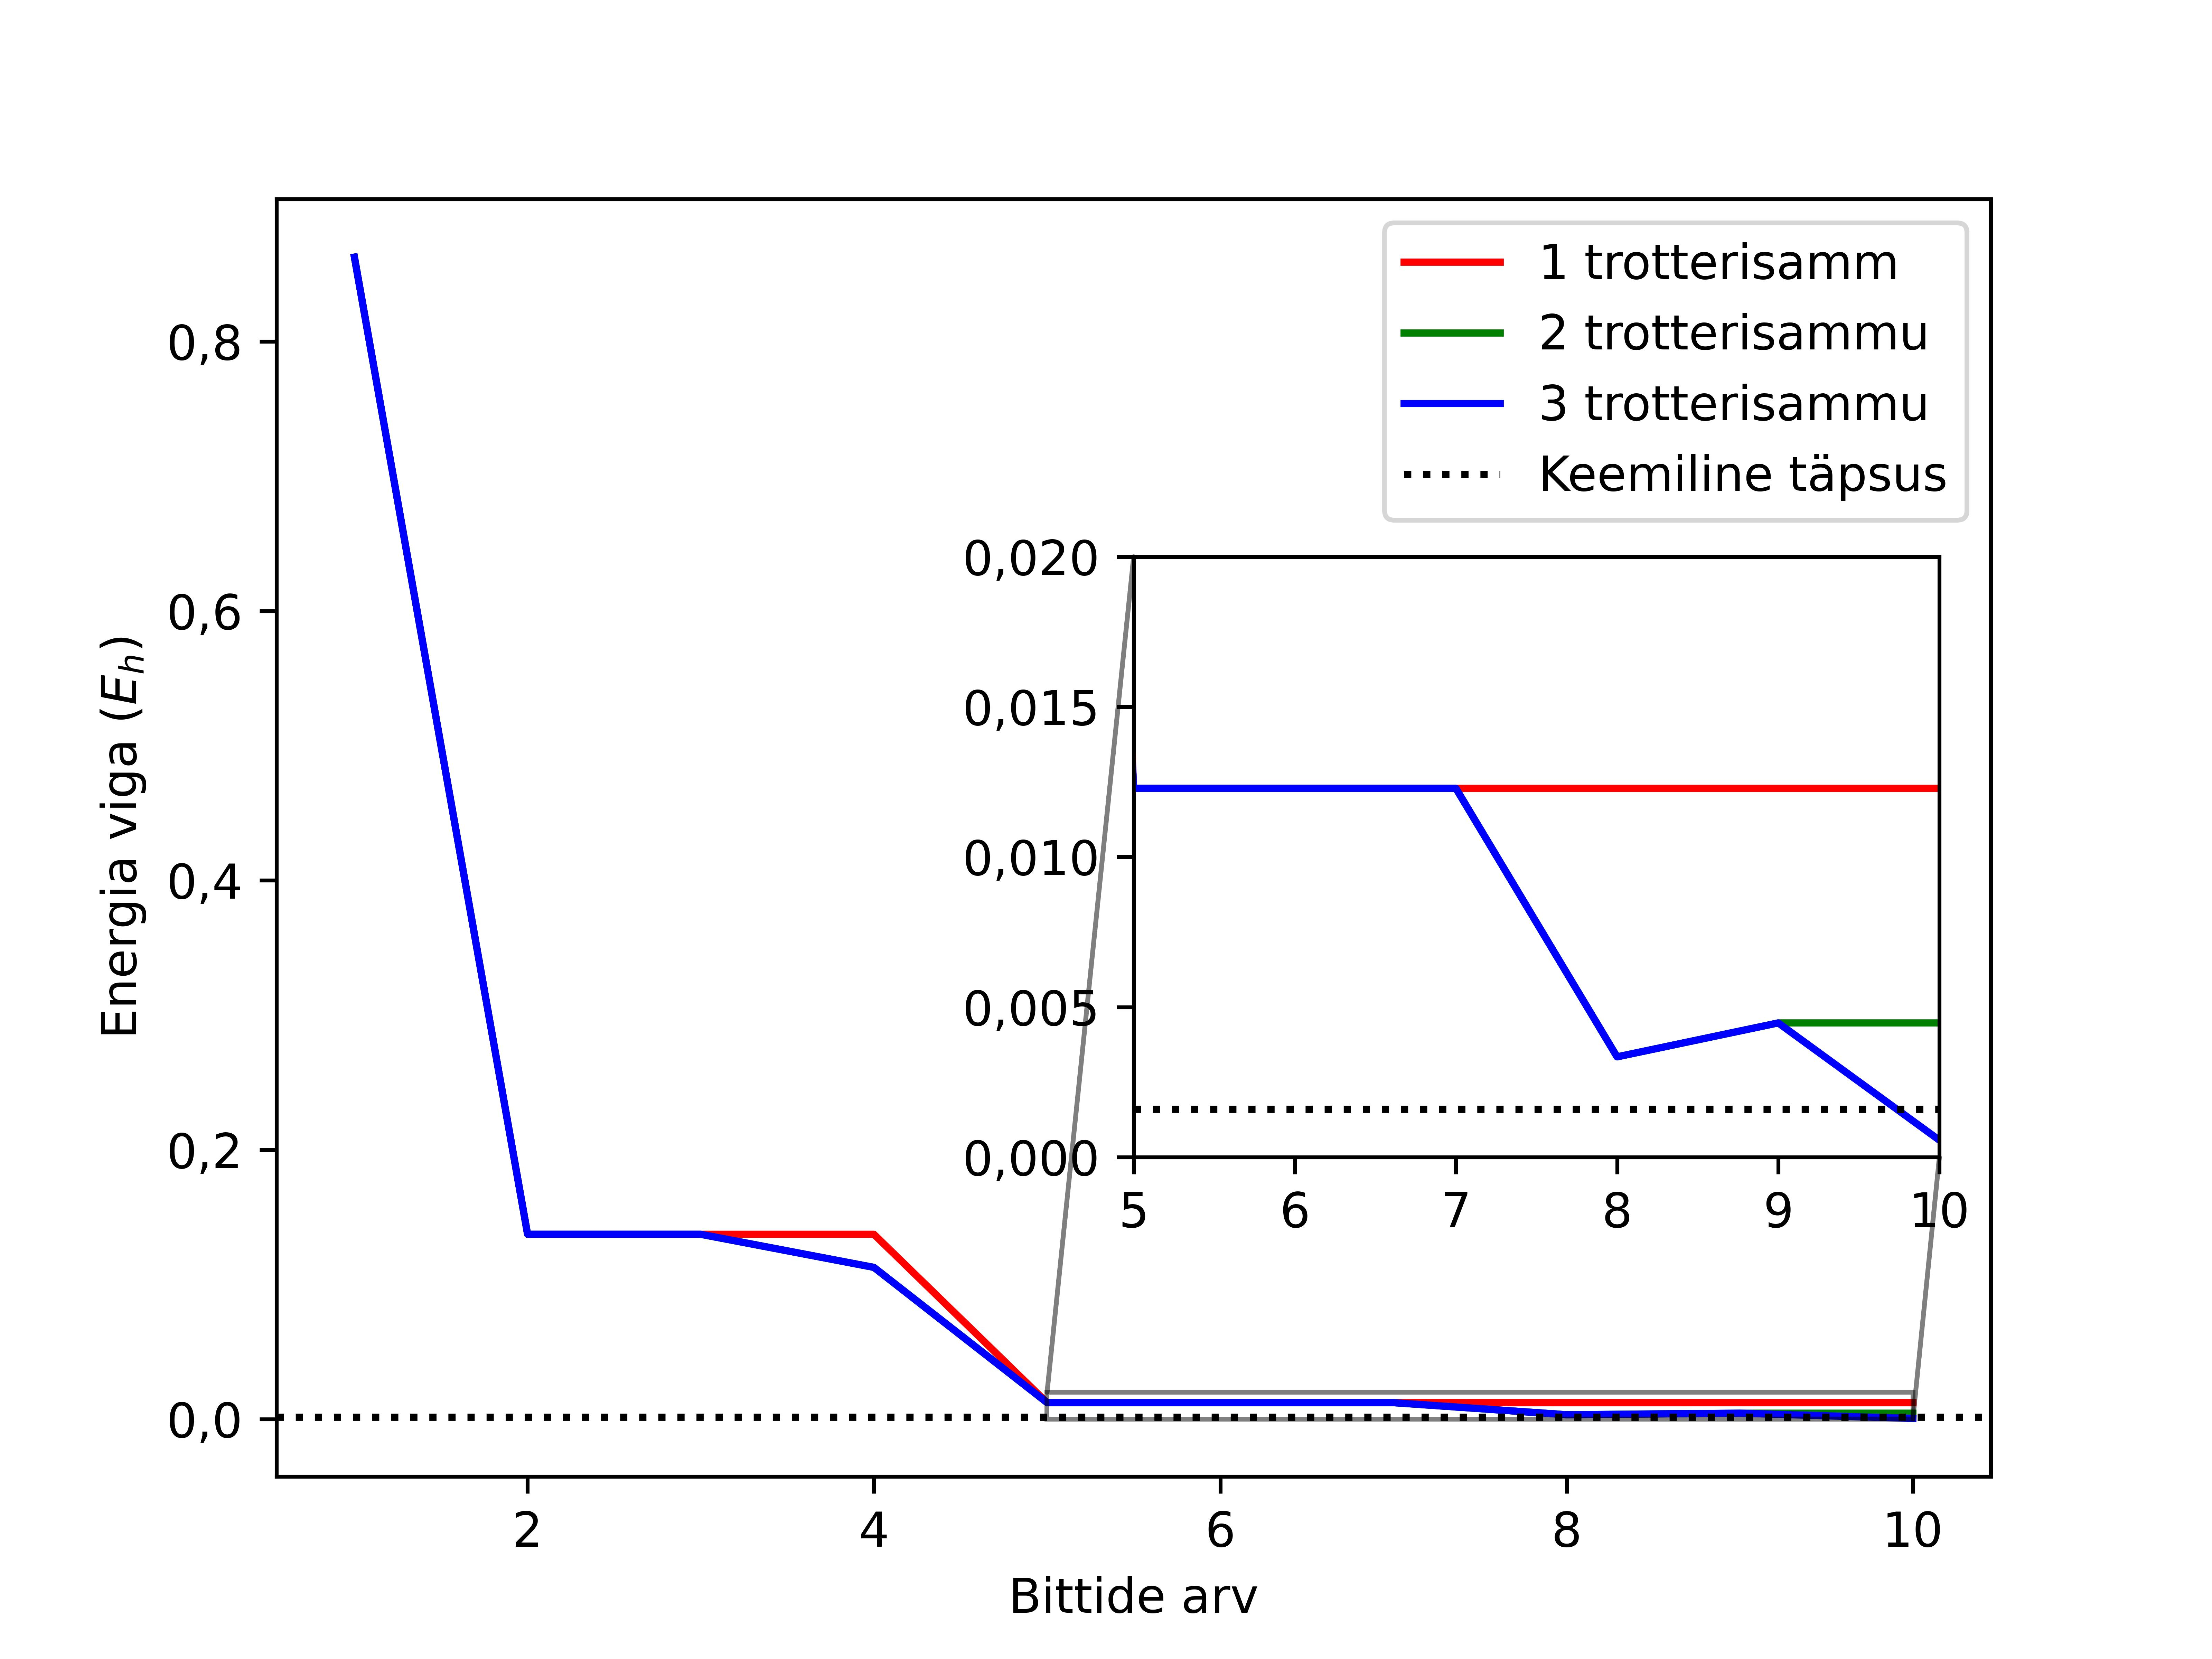
\includegraphics{trotsteps.jpg}
    \caption{Energia hinnangu sõltuvus bittide arvust. Pandagu tähele, et roheline joon on peaaegu täielilt sinese joone taga varjatud}
    \label{fig:trotsteps}
\end{figure}

Nagu näha jooniselt~\ref{fig:trotsteps} langevad ühe-, kahe- ja kolme-trotterisammused energia hinnangud hästi kokku juhul, kui energiat hinnata kahekse- või vähemakvantbitise täpsuega.
Erinevused ilmnevad alles kahekast kvantbitist suurema täpsuse juures.
Keemiline täpsuse saavutasime kolme trotterisammu ja kümne kvantbitiga.

Parimal juhul on võimalik saavutada vaid nii suur täpsus, kui keemilise baasi valik lubab.

Kvantbittide arvust sõltub käitamisaeg kahte moodi.
Esiteks, rohkem kvantbitte tähendab pikemat käitamisaega.
Teiseks, kui faasi hindamiseks kasutada rohkem kvantbitte, siis kasvab eksponentsiaalselt ka ahela pikkus.

\begin{figure}[h]
    \centering
    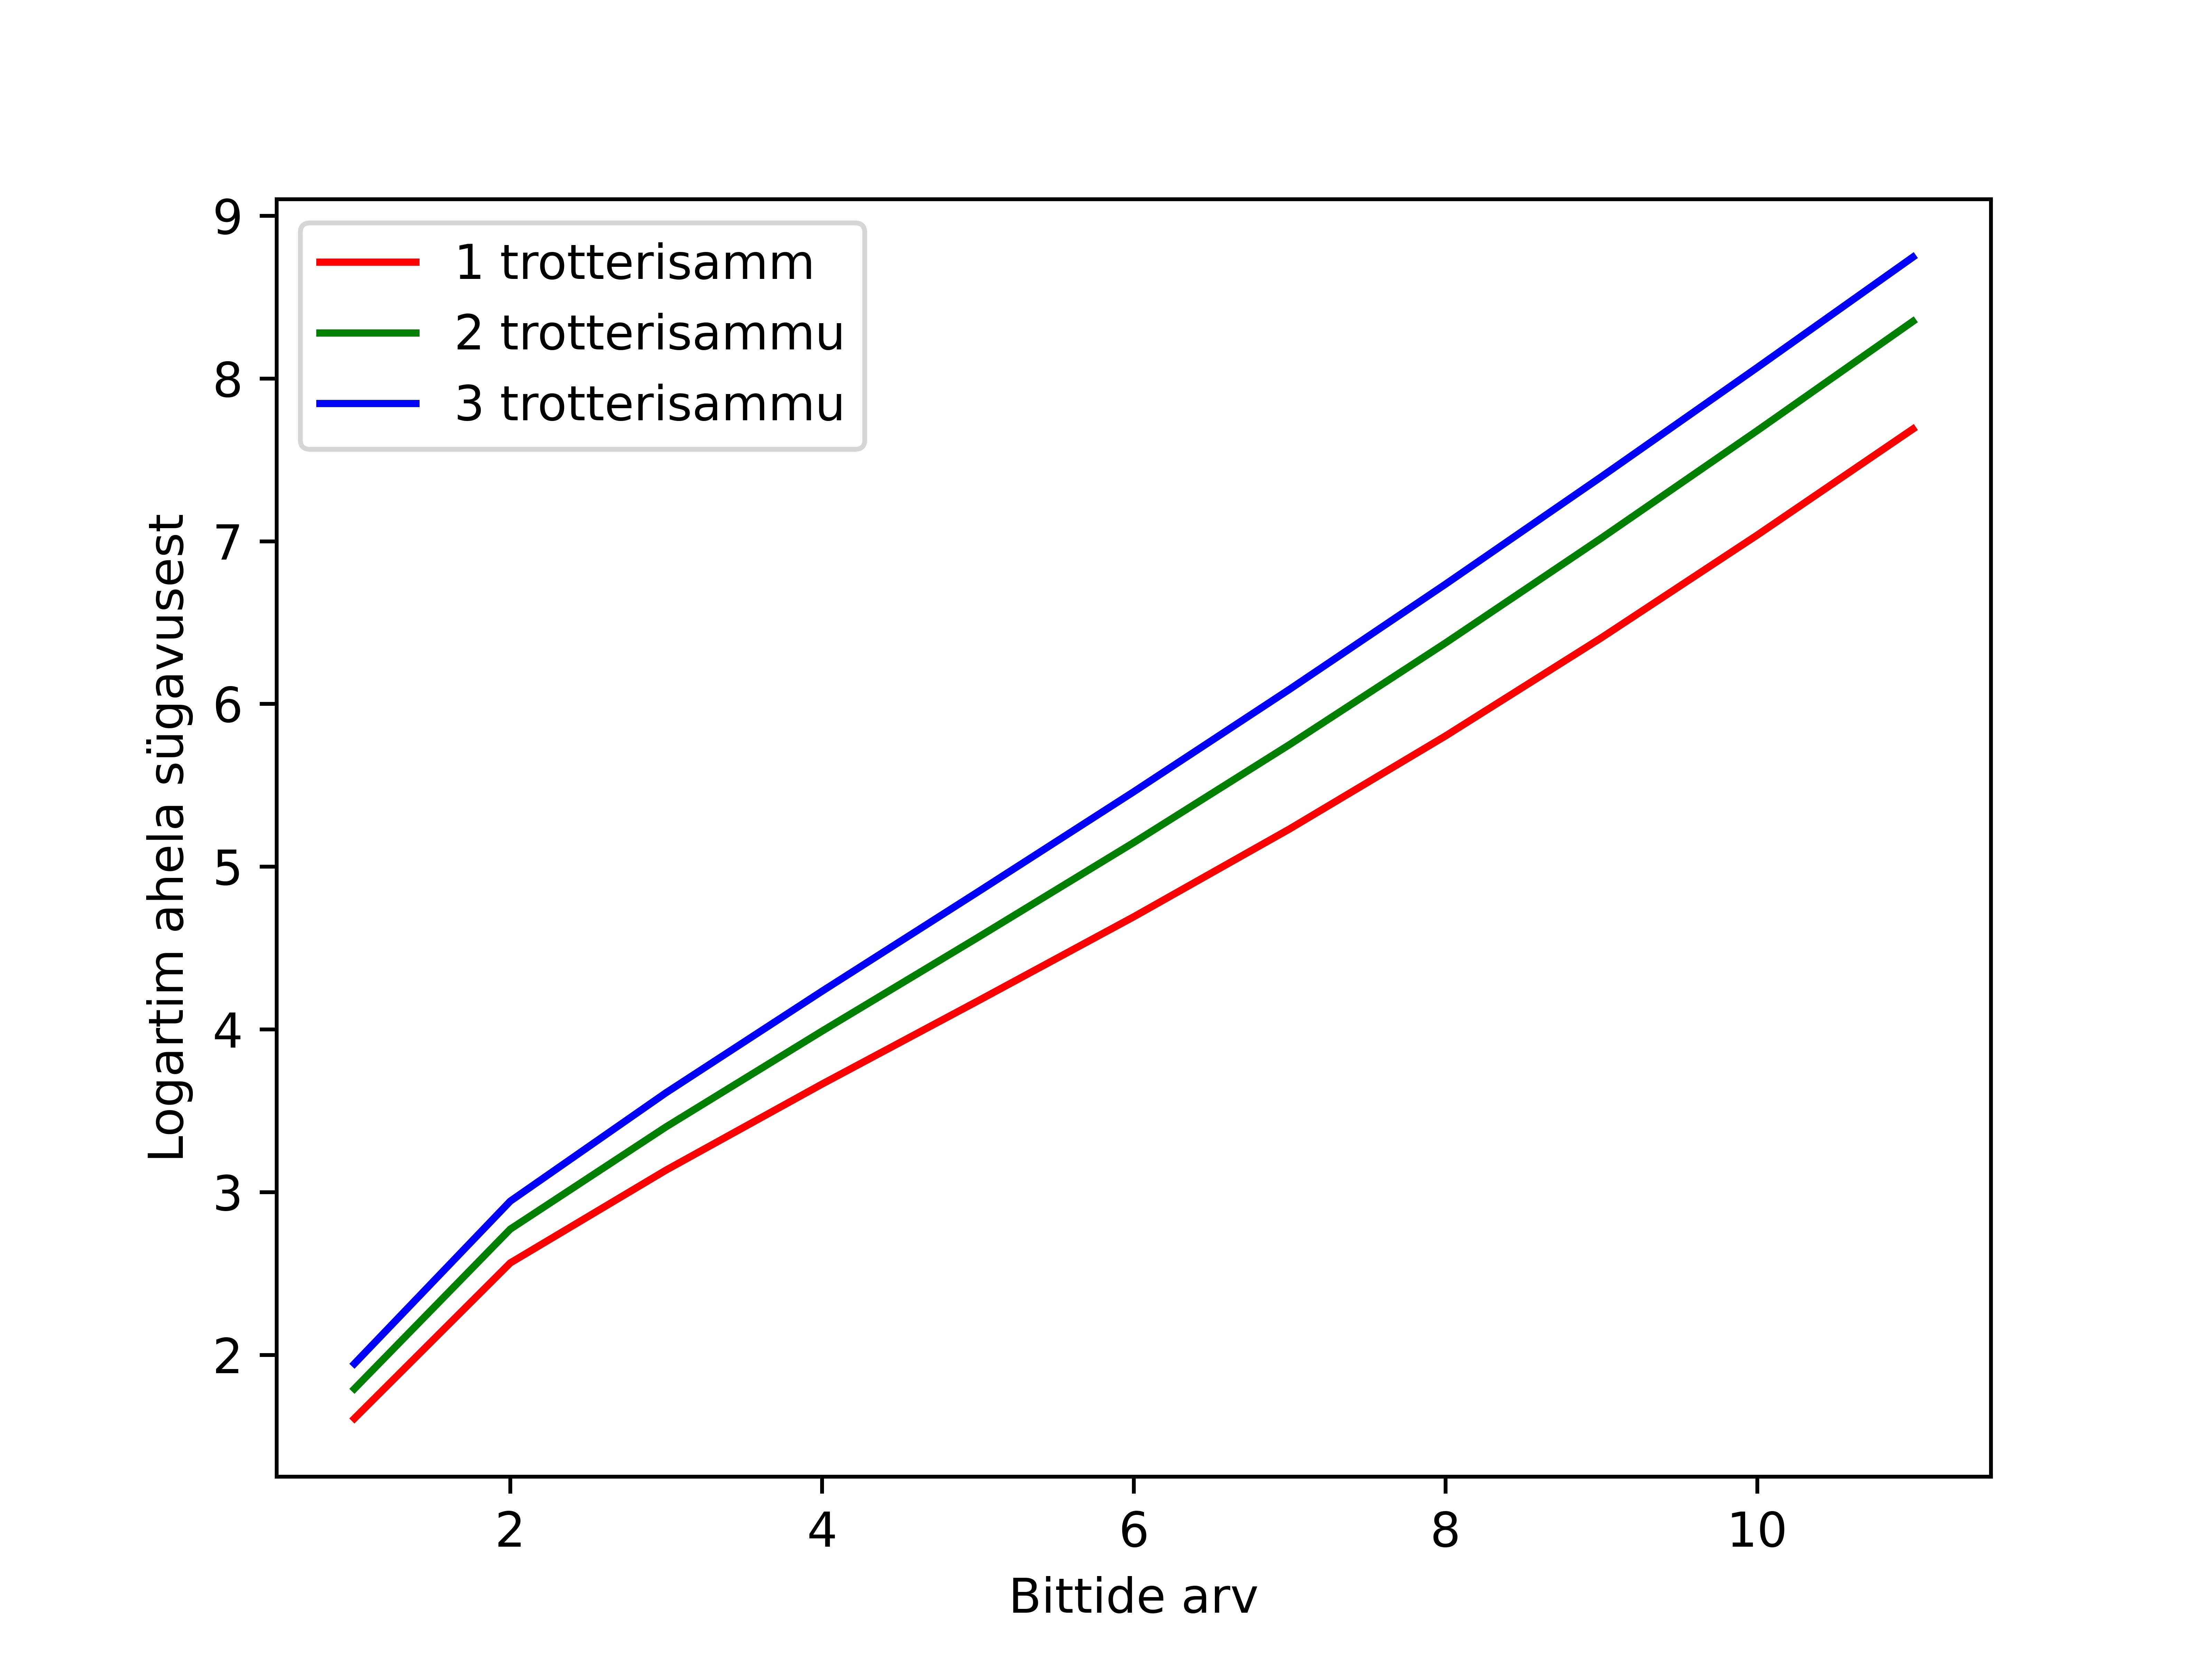
\includegraphics{depths.jpg}
    \caption{Ahela sügavuse sõltuvs bittide arvust}
    \label{fig:depths}
\end{figure}

Joonisel~\ref{fig:depths} on näidatud ahela sügavuse, st ahela kvantväravate arvu, sõltuvus faasi hindamise registri suurusest erinevate trotterisammude arvu jaoks.
Praktiliselt oli teostatav kümnekvantbitise faasi hindamise registri kasutamine.

\section{Eneriga piirväärtus}

Samuti sõltub energia hinnangu täpsus energia piirväärtuse valikust, mida kujutab joonis~\ref{fig:bounds}.

\begin{figure}[h]
    \centering
    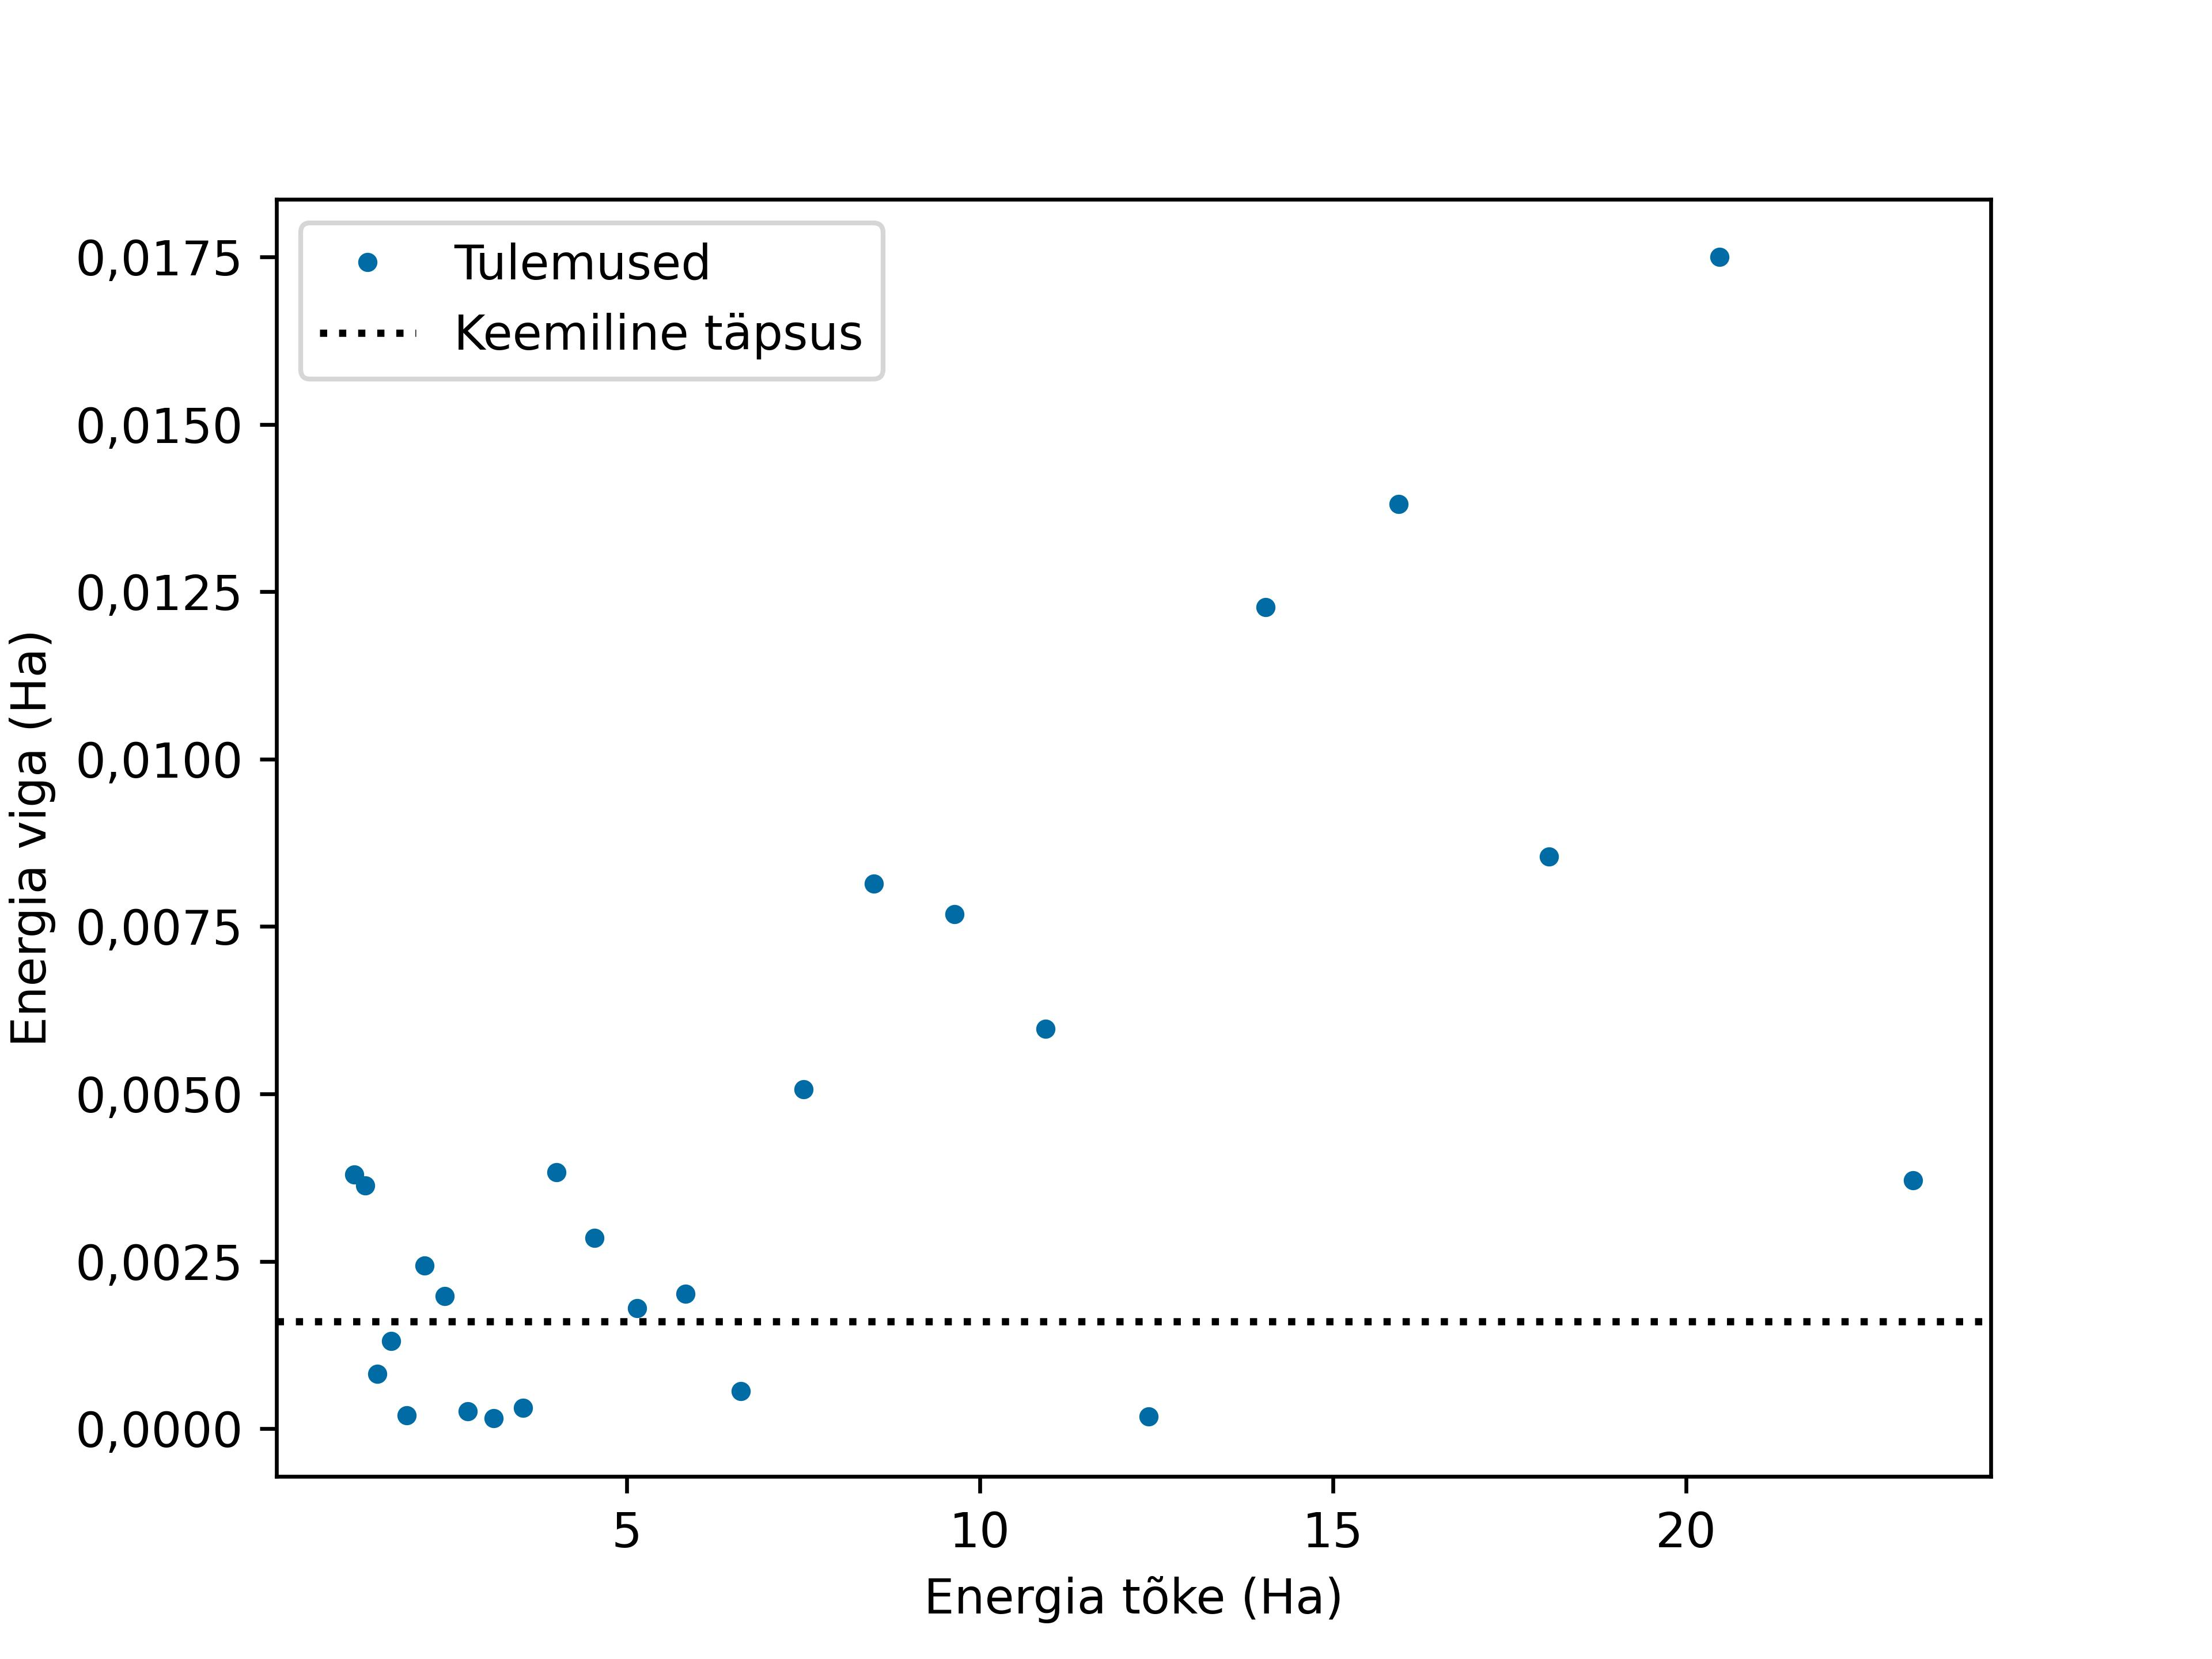
\includegraphics{bounds.jpg}
    \caption{Energia hinnagu sõltuvus energia piirväärtuse valikust}
    \label{fig:bounds}
\end{figure}

Nagu näha, sõltub energia hinnagu täpsus piirvääruse valikust kaootiliselt.
Siiski energiast oluliselt suuremate piirväärtuste puhul (mida joonisel~\ref{fig:bounds} pole kujutatud), täpsus reeglina väheneb.
Nimelt on sellisel juhul \(\phi \ll 1\) ja seega ei panusta esimesed kvantbitid tulemuse täpsusesse.

\section{Edasiarendusi}

Faasi hindamise algoritmi peamine edasiarendus on iteratiivne faasi hindamise algoritm~\cite{mcardle+etal, omalley+etal}.

Tegemist on hübriidalgoritmiga, mis kasutab klassikalist ja kvantarvutit vaheldumisi.
Kvantarvutuslikult loetakse välja üks bitt korraga, mille põhjal koostatakse klassikaliselt uus ahel järgmise biti välja lugemiseks.

Sellise algoritmi eeliseks on, et faasi hindamise registrisse on vaja vaid ühte kvantbitti.
Samuti on ahelad lühemad.

Puuduseks on keerulisus ja asjaolu, et võimalik viga mõne biti välja lugemisel võib kumuleeruda.

\printbibliography[heading=bibintoc, title=Kirjandus]

\end{document}
